\documentclass{article}
\usepackage{graphicx}
\usepackage[english]{babel}
\usepackage{verbatim} % for multi line comments
\usepackage{xcolor}
\usepackage[sfdefault]{roboto}
\usepackage[a4paper, total={6in, 8in}]{geometry}
\usepackage{hyperref}
\hypersetup{
    colorlinks,
    citecolor=black,
    filecolor=black,
    linkcolor=black,
    urlcolor=black
}

\graphicspath{{../Images}}



% \bibliographystyle{6}
\begin{document}

\begin{titlepage}
  \centering
    \vfill
    {\bfseries\Huge
	    Scope \& Methodology
        \vskip2cm
      }
      {\bfseries\Large
        Jayden Weverink
        \vskip0cm
      }
      {\bfseries\Large
        Jordy van der List
        \vskip0cm
      }
      {\bfseries\Large
        Michael Francis
        \vskip0cm
      }
      {\bfseries\Large
        Tim Wolcken
        \vskip0cm
      }
      {\bfseries\Large
        Rafael Bieze
        \vskip0cm
      }
      {
        \bfseries\normalsize
        %176-671\\
        \vskip1cm
        \today\\
    }
    \vfill
    
\includegraphics[width=4cm]{logohr.png} % also works with logo.pdf
    \vfill
    \vfill
\end{titlepage}
\newpage
\tableofcontents

\setlength{\parindent}{0em}
\setlength{\parskip}{1em}
\flushleft

% \clearpage %====================================================================
\section{Introduction}


\clearpage %====================================================================
\section{Scope}

The scope described what data had to be collected, what data was not collected and the reasoning behind these decisions.

For the research only Android applications were tested, the reason behind this was that the necessary tools that were provided only work on Android applications. 
This means that no IOS applications were tested. 
Another reason that iOS applications were not tested was that they could not be installed on an emulator on Windows operating systems, 
while android applications could be installed on Unix systems (also includes MAC OS) and Windows systems.

To understand how the application worked the decision has been made to preform a behavior analysis. 
During this analysis only visual data of the application was collected. 
The research does not require the collection of any form of background activities performed by the application during the behavior analysis. 
These activities did not hold value for the behavior analysis.

It was decided that a network analysis was necessary to raise the probability of retrieving the information that the research required. 
During this analysis all sources that the applications connected to were collected. These sources could consist of IP-addresses and domain names. 
The research allowed for the gathering of information of any potential servers with the use of tools such as shodan.io. 
Connecting to these services however fell outside the scope of the research. This had the potential of raising unwanted attention of the malicious parties.

For the proper analysis of an Android application it was decided that doing a code analysis was essential, 
the code had potential to had revealed a lot of important information about what the application was doing that would otherwise have been very hard to find. 
It had been important for the code analysis to get ahold of the source code of the software. 
This was achieved by using a decompiling program if the source of the application was not available.

To further understand the application the decision has been made that a process analysis was required. 
During this analysis, the memory and the processes that had been activated in the background were monitored. 
The different dependencies that the application used, had also been monitored.

During a reasearch like this there is a chance that the malicious application uses a command and control server. 
This created a chance to potentially gain access to the server or database. It was decided that the actions within the research were within the confounds of the law. 
For this reason, it was crucial for the research that the international laws were being upheld. 
One of these laws had prohibited the research from interfering or tampering with the server or database without the express consent of the other party. 
Because of this reason, it was decided that there would be made notes about the connection and not interact with it in any way.

\newpage
\section{Methodology}

For proper analysis of an android application a testing environment has to be configured.
Each member had chosen to either work in a virtual machine or use their local machine to test the application.
Using a local machine, every member must consider their own safety when working with malicious software.
Publicly available tools were also properly setup on the local or virtual machine such as Android Studio, mitmproxy and Wireshark.

\subsection{Finding the malicious applications}

For the research it was decided that all the selected applications had come from the site Koodous and had confirmed to be malicious with the site VirusTotal.
This had been done individually by all team members to find applicable APK files for the research.
Some checks were performed manually to see if the applications contained any pointers that indicated that they contained malware.
The application was checked on its availability for download on the Google Play store.
The potentially malicious application was compared with the variant from the Google Play store.
A few examples of these pointers were differing sizes or if both had the exact same package name as the Google Play store variant while differing in permissions or certificates.
If it had one of those pointers, then it likely was an indicator that there was something extra hidden in the code.

The application was retrieved from both Koodous and the Google Play Store.
The APK from Google Play was downloaded using the apkcombo.com website.
Both APK files were uploaded to VirusTotal to check for any differences in permissions between the two versions of the application.
Anything VirusTotal had marked as malicious, was noted.
It was up to the discretion of each individual team member to decide on the application they wanted to work on for the duration of the project.

\subsection{Behavior analysis}

The research required that each team member had one application to examine.
This had been done on a virtual computer, with android studio installed, or locally.
During the installation of the application the network traffic was captured.
This was done using Wireshark and mitmproxy.
The network traffic was not relevant for the behavior analysis but was captured as part of the network analysis.

The behavior analysis was predominantly about using the application from a users point of view and noting anything out of the ordinary.
This was also compared step by step to the original (non-malicious) application.
The differences between the two were noted for further investigative purposes.
The ordinary behavior was investigated further during network and code analysis.

\subsection{Network analysis}

During the behavior analysis the network traffic from the application was captured using Wireshark and mitmproxy.
During the network analysis this captured network traffic was analyzed using a combination of Wireshark, mitmproxy and shodan.io.
Wireshark was used to capture all network data that was sent by the application and gave the opertunity to perform a deep analysis what exactly was sent.
Mitmproxy was used to capture all http and https requests, this was used to find what IP-addresses connections were made to.
During the analysis anything that stood out like any IP addresses and or domain names were written down.

Shodan.io was used for analyzing the IP addresses and domain names found with Wireshark and mitmproxy.
Wireshark and mitmproxy were able to reveal all the network traffic sent and received by the application.
Shodan.io revealed the other functions of the servers and whether there are similar servers, perhaps from the same hosting provider.

\subsection{Code analysis}

For the code analysis, JadX and Dex2Jar were used to decompile the application. Both of these applications were used to review the code. This allowed us to double-check the code and make sure the decompiled APK's code was accurate. Analyzing the code was very difficult due to obfuscation. Where possible it was documented whether the code was malicious or not.

\subsection{Process analysis}
The Processes were analyzed to gain the insights that the research needs.
The application was started in the emulator of Android Studio.
During the startup and use of the application, the Memory profiler was used to monitor the memory usage of the application.
All memory usage was documented and all peculiar behavior had been investigated further, to understand what had caused the suspicious behavior.
Optionally, a heap dump was done during execution, which led to interesting findings.

\subsection{Countermeasures and detection}

To finalize the analysis, a YARA ruleset had been created for the application.
To inform end users, methods have been documented that the end user can apply to mitigate the effects of the malicious code.
All findings were documented into a report which was delivered to the team leader.
These steps were performed by all the members.
If an application needed additional steps this was declared at the start of the application chapter.


\newpage
\section{<application name> Application Analysis by Jayden}

<should include application name, version numbers, apk size>

\newpage
\subsection{VirusTotal summary}

<should include, how many times marked malicious, package name and any other interesting things>

\subsubsection{Permission requests}

<permissions requested by the app (can be found on virus total)>

\newpage
\subsection{Behavior analysis}

<what does the app behave like when installed and ran>

\newpage
\subsection{Network analysis}

<what does the network traffic look like>

\subsubsection{HTTP proxy analysis}

<what did the proxy reveal about the network traffic>

\subsubsection{Wireshark analysis}

<what did WireShark reveal about the network traffic>

\subsubsection{Reconnaissance [optional]}

<what was found using shodan.io>

\newpage
\subsection{Code analysis}

<interesting stuff found in code>

\newpage
\subsection{Process analysis}

<interesting stuff found in the process and memory, etc.>

\newpage
\subsection{Countermeasures and detection}

\subsubsection{Preventive measures}


<Measures to prevent installing this application>

\subsubsection{Detective measures}

<Measures to detect if this application is installed>

\subsubsection{Reactive measures}

<What to do if it is installed>

\subsubsection{YARA rule set}

<A YARA rule set created based on your findings>


\newpage
\section{Firefox Application Analysis by Jordy}
The malicious application that was analyzed in this chapter had the name "FireFox".
This application was found on \href{https://koodous.com/apks/26a7576cc1182bf90fb16c3320d12a736b3faa10c158755605f36daae4b197b7}{Koodous} with the package name “com.eset.ems2.gp” and with version number 85.1.3.
The size of this application was 70.4 MB.
To confirm that this application was actually malicious a search on the \href{https://play.google.com/store/apps/details?id=org.mozilla.firefox&hl=nl&gl=US}{Google Play Store} was performed.
The current official version of Mozilla Firefox is 94.1.2.
To get the official Firefox version 85.1.3 it was necessary to download the application from another source.
The APK file was checked with \href{https://www.virustotal.com/gui/file/59ce0f9ea256b4576f391d01c685ced2db224a252bf09c3f362e6859a6c7ead5/details}{VirusTotal} and compared to the most recent official version of Mozilla Firefox.
This process has been described in detail in chapter 4.1.

The official APK file for Mozilla Firefox version 85.1.3 had the package name “org.mozilla.firefox” and had the size of 63.39 MB.
All aspects were relatively similar been the versions 85.1.3 and 94.1.2 of Mozilla Firefox with a few small alterations.
These alterations were because one of the versions was a few months older.

From this moment onwards in the chapter the “official application” will be referring to the 85.1.3 version of Mozilla Firefox with the package name “org.mozilla.firefox” and the “malicious application” will be referring to the APK file found on Koodous with the package name “com.eset.ems2.gp”.

\newpage
\subsection{VirusTotal summary}
The selected malicious application was checked on VirusTotal for an overview of the application.
On this website it is possible to see if security vendors flag this application as malicious, what permissions the application asks for, the package name and many more aspects of the application.
With this information both of the applications were compared with each other.
In this chapter the process and results are described.

\subsubsection{Security vendor flags}
VirusTotal indicated that the malicious application was marked as malicious by 25 out of 61 security vendors.
In the table under this paragraph all flags are described.

\begin{tabular}{|l|l|}
    \hline
    \textbf{Security vendor} & \textbf{Flag}                        \\ \hline
    AegisLab                 & Trojan.AndroidOS.Agent.C!c           \\ \hline
    AhnLab-V3                & Trojan/Android.Agent.449065          \\ \hline
    Avast                    & Android:Agent-RSY {[}Trj{]}          \\ \hline
    Avast-Mobile             & Android:Evo-gen {[}Trj{]}            \\ \hline
    AVG                      & Android:Agent-RSY {[}Trj{]}          \\ \hline
    BitDefenderFalx          & Android.Trojan.SpyAgent.P            \\ \hline
    CAT-QuickHeal            & Android.Agent.ADV                    \\ \hline
    Comodo                   & Malware@\#2ldj5q9ll943m              \\ \hline
    Cyren                    & AndroidOS/Trojan.GMOM-2              \\ \hline
    DrWeb                    & Android.Spy.516.origin               \\ \hline
    ESET-NOD32               & A Variant Of Android/Spy.Agent.BAY   \\ \hline
    F-Secure                 & Malware.ANDROID/SMSAgent.FHAL.Gen    \\ \hline
    Fortinet                 & Android/Agent.AZF!tr.spy             \\ \hline
    K7GW                     & Spyware ( 00516e5c1)                 \\ \hline
    Kaspersky                & HEUR:Trojan-Spy.AndroidOS.Agent.vp   \\ \hline
    McAfee                   & ANDROID/Spy.d                        \\ \hline
    McAfee-GW-Edition        & ANDROID/Spy.d                        \\ \hline
    Microsoft                & Trojan:AndroidOS/Spynote.B!MTB       \\ \hline
    NANO-Antivirus           & Trojan.Android.Hidden.estanm         \\ \hline
    Sangfor Engine Zero      & Malware.Android-Script.Save.dc318d22 \\ \hline
    Sophos                   & Andr/Xgen2-EQ                        \\ \hline
    Symantec Mobile Insight  & Trojan:Malapp                        \\ \hline
    Trustlook                & Android.Malware.General (score:9)    \\ \hline
    Yandex                   & Trojan.Mober.bTTGwd.156              \\ \hline
    ZoneAlarm by Check Point & HEUR:Trojan-Spy.AndroidOS.Agent.vp   \\ \hline
\end{tabular}

These flags from the different security vendors clearly indicate that the malicious application is in fact malicious and most likely a Trojan.

A Trojan is a blanket term for malicious software that disguises itself as a harmless application.
\newpage
\subsubsection{Permission requests}
Every application asks for permission when you install it on a phone.
In this subchapter the permissions that the official and malicious applications asked for are described.
\subsubsubsection{Malicious application permissions}
The malicious application asked for the following permissions:

\texttt{android.permission.PROCESS\_OUTGOING\_CALLS}
\newline \texttt{android.permission.ACCESS\_COARSE\_LOCATION}
\newline \texttt{android.permission.BLUETOOTH}
\newline \texttt{android.permission.INTERNET}
\newline \texttt{android.permission.WRITE\_CONTACTS}
\newline \texttt{android.permission.SEND\_SMS}
\newline \texttt{android.permission.WRITE\_CALL\_LOG}
\newline \texttt{android.permission.READ\_CALL\_LOG}
\newline \texttt{com.android.browser.permission.READ\_HISTORY\_BOOKMARKS}
\newline \texttt{android.permission.WRITE\_EXTERNAL\_STORAGE}
\newline \texttt{android.permission.RECORD\_AUDIO}
\newline \texttt{android.permission.ACCESS\_FINE\_LOCATION}
\newline \texttt{android.permission.CALL\_PHONE}
\newline \texttt{android.permission.READ\_PHONE\_STATE}
\newline \texttt{android.permission.READ\_SMS}
\newline \texttt{android.permission.SYSTEM\_ALERT\_WINDOW}
\newline \texttt{android.permission.CAMERA}
\newline \texttt{android.permission.CHANGE\_WIFI\_STATE}
\newline \texttt{android.permission.RECEIVE\_SMS}
\newline \texttt{android.permission.READ\_CONTACTS}
\newline \texttt{android.permission.INSTALL\_PACKAGES}
\newline \texttt{android.permission.ACCESS\_WIFI\_STATE}
\newline \texttt{android.permission.SET\_WALLPAPER\_HINTS}
\newline \texttt{android.permission.ACCESS\_NETWORK\_STATE}
\newline \texttt{android.permission.SET\_WALLPAPER}
\newline \texttt{android.permission.READ\_EXTERNAL\_STORAGE}
\newline \texttt{android.permission.RECEIVE\_BOOT\_COMPLETED}
\newline \texttt{android.permission.WRITE\_SETTINGS}
\newline \texttt{android.permission.VIBRATE}
\newline \texttt{android.permission.KILL\_BACKGROUND\_PROCESSES}
\newline \texttt{android.permission.WAKE\_LOCK}
\newline \texttt{android.permission.GET\_ACCOUNTS}

A lot of these permissions are not usually asked for by an internet browser.
An in depth comparison of the differences between the applications permissions was described in detail in chapter 4.1.2.3.
\newpage
\subsubsubsection{Official application permissions}
The official application asked for the following permissions:

\texttt{android.permission.READ\_EXTERNAL\_STORAGE }
\newline \texttt{android.permission.WRITE\_EXTERNAL\_STORAGE }
\newline \texttt{android.permission.USE\_BIOMETRIC }
\newline \texttt{android.permission.RECEIVE\_BOOT\_COMPLETED}
\newline \texttt{android.permission.USE\_FINGERPRINT }
\newline \texttt{android.permission.ACCESS\_WIFI\_STATE}
\newline \texttt{com.android.launcher.permission.INSTALL\_SHORTCUT }
\newline \texttt{com.google.android.c2dm.permission.RECEIVE}
\newline \texttt{com.google.android.finsky.permission.BIND\_GET\_INSTALL\_REFERRER\_SERVICE}
\newline \texttt{android.permission.MODIFY\_AUDIO\_SETTINGS }
\newline \texttt{android.permission.DOWNLOAD\_WITHOUT\_NOTIFICATION}

An in depth comparison of the differences between the applications permissions was described in detail in chapter 4.1.2.3.
\newpage
\subsubsubsection{Differences between permissions}
The malicious application asked for the following permissions that the official application did not ask for:

\texttt{android.permission.PROCESS\_OUTGOING\_CALLS}
\newline \texttt{android.permission.ACCESS\_COARSE\_LOCATION}
\newline \texttt{android.permission.BLUETOOTH}
\newline \texttt{android.permission.INTERNET}
\newline \texttt{android.permission.WRITE\_CONTACTS}
\newline \texttt{android.permission.SEND\_SMS}
\newline \texttt{android.permission.WRITE\_CALL\_LOG}
\newline \texttt{android.permission.READ\_CALL\_LOG}
\newline \texttt{com.android.browser.permission.READ\_HISTORY\_BOOKMARKS}
\newline \texttt{android.permission.RECORD\_AUDIO}
\newline \texttt{android.permission.ACCESS\_FINE\_LOCATION}
\newline \texttt{android.permission.CALL\_PHONE}
\newline \texttt{android.permission.READ\_PHONE\_STATE}
\newline \texttt{android.permission.READ\_SMS}
\newline \texttt{android.permission.SYSTEM\_ALERT\_WINDOW}
\newline \texttt{android.permission.CAMERA}
\newline \texttt{android.permission.CHANGE\_WIFI\_STATE}
\newline \texttt{android.permission.RECEIVE\_SMS}
\newline \texttt{android.permission.READ\_CONTACTS}
\newline \texttt{android.permission.INSTALL\_PACKAGES}
\newline \texttt{android.permission.SET\_WALLPAPER\_HINTS}
\newline \texttt{android.permission.ACCESS\_NETWORK\_STATE}
\newline \texttt{android.permission.SET\_WALLPAPER}
\newline \texttt{android.permission.WRITE\_SETTINGS}
\newline \texttt{android.permission.VIBRATE}
\newline \texttt{android.permission.KILL\_BACKGROUND\_PROCESSES}
\newline \texttt{android.permission.WAKE\_LOCK}
\newline \texttt{android.permission.GET\_ACCOUNTS}

\newpage
There were a lot of interesting permission that the malicious application asked for that the official application did not ask for.
Most of these permissions are never necessary for a web browser to have. The permissions were described in different groups.

\textbf{Calls, SMS, accounts and contacts:}
A web browser would never need to have access to a call log, any of your accounts, contacts or SMS messages.
There would also never be a need for Firefox to make a phone call or send a SMS message on its own.

\texttt{android.permission.PROCESS\_OUTGOING\_CALLS}
\newline \texttt{android.permission.WRITE\_CONTACTS}
\newline \texttt{android.permission.SEND\_SMS}
\newline \texttt{android.permission.WRITE\_CALL\_LOG}
\newline \texttt{android.permission.READ\_CALL\_LOG}
\newline \texttt{android.permission.CALL\_PHONE}
\newline \texttt{android.permission.READ\_SMS}
\newline \texttt{android.permission.RECEIVE\_SMS}
\newline \texttt{android.permission.READ\_CONTACTS}
\newline \texttt{android.permission.GET\_ACCOUNTS}

\textbf{Bluetooth, network and Location:}
A web browser like Firefox has no need for Bluetooth permissions.
Furthermore no application should need to access or change the Wi-Fi state of a phone.
A connection with the internet should have been enough.
The application should never have asked for access to location at all times.
This permission might get asked by a very select few websites.
This does not mean a internet browser needs to have this permission when it gets installed. 

\texttt{android.permission.BLUETOOTH}
\newline \texttt{android.permission.INTERNET}
\newline \texttt{android.permission.ACCESS\_NETWORK\_STATE}
\newline \texttt{android.permission.CHANGE\_WIFI\_STATE}
\newline \texttt{android.permission.ACCESS\_FINE\_LOCATION}
\newline \texttt{android.permission.ACCESS\_COARSE\_LOCATION}

\textbf{Audio and video:}

A web browser would only need to have access to your camera or microphone when someone would be on a website like zoom.
It should have never asked for these permissions during the installation. 

\texttt{android.permission.CAMERA}
\newline \texttt{android.permission.RECORD\_AUDIO}

\newpage
\textbf{Phone functions:}

Most of these permissions are permissions that no web browser would ever need.
The install packages, write settings and kill background processes are a few examples of unnecessary permissions that could ruin your Android OS when the wrong applications use them.
An example of a not harmful but unnecessary permission was the vibrate permission.
Firefox would never need to have access to that permission.

\texttt{android.permission.READ\_PHONE\_STATE}
\newline \texttt{android.permission.SYSTEM\_ALERT\_WINDOW}
\newline \texttt{android.permission.INSTALL\_PACKAGES}
\newline \texttt{android.permission.KILL\_BACKGROUND\_PROCESSES}
\newline \texttt{android.permission.WRITE\_SETTINGS}
\newline \texttt{android.permission.SET\_WALLPAPER}
\newline \texttt{android.permission.SET\_WALLPAPER\_HINTS}
\newline \texttt{android.permission.VIBRATE}
\newline \texttt{android.permission.WAKE\_LOCK}

\subsubsection{Relations}
On the VirusTotal website it was shown that the malicious application has made a connection to two IP addresses.
These IP addresses are:

\texttt{3.134.39.220}
\newline \texttt{3.14.182.203}

These IP addresses were described in the network analysis chapter.

\newpage
\input{individual/jordy/Behavior Analysis}

\newpage
\subsection{Network analysis}
To get a better understanding of the network traffic behind the malicious application a network analysis was performed.
The process and results of the network analysis are described in this chapter.

\subsubsection{HTTP proxy analysis}
Mitmproxy was used to capture the network traffic to and from the emulated phone.
Mitmproxy ended up showing that the phone made a connection with multiple different IP addresses.
After around 30 minutes of capturing the network traffic it kept connecting and disconnecting with the same 5 IP addresses.
A couple of times an IP address came up that was in a completely different range of IP’s.

In the picture that is shown below there are a total of 8 IP addresses that are captured again and again.
5 out of the 8 IP addresses all started with a 3.
The remaining IP addresses were very different from the 3. range and they were not consistently looping like the others.
In mitmproxy there was not a lot of information that could be analyzed with the software.

\begin{figure}[H]
    \centering
    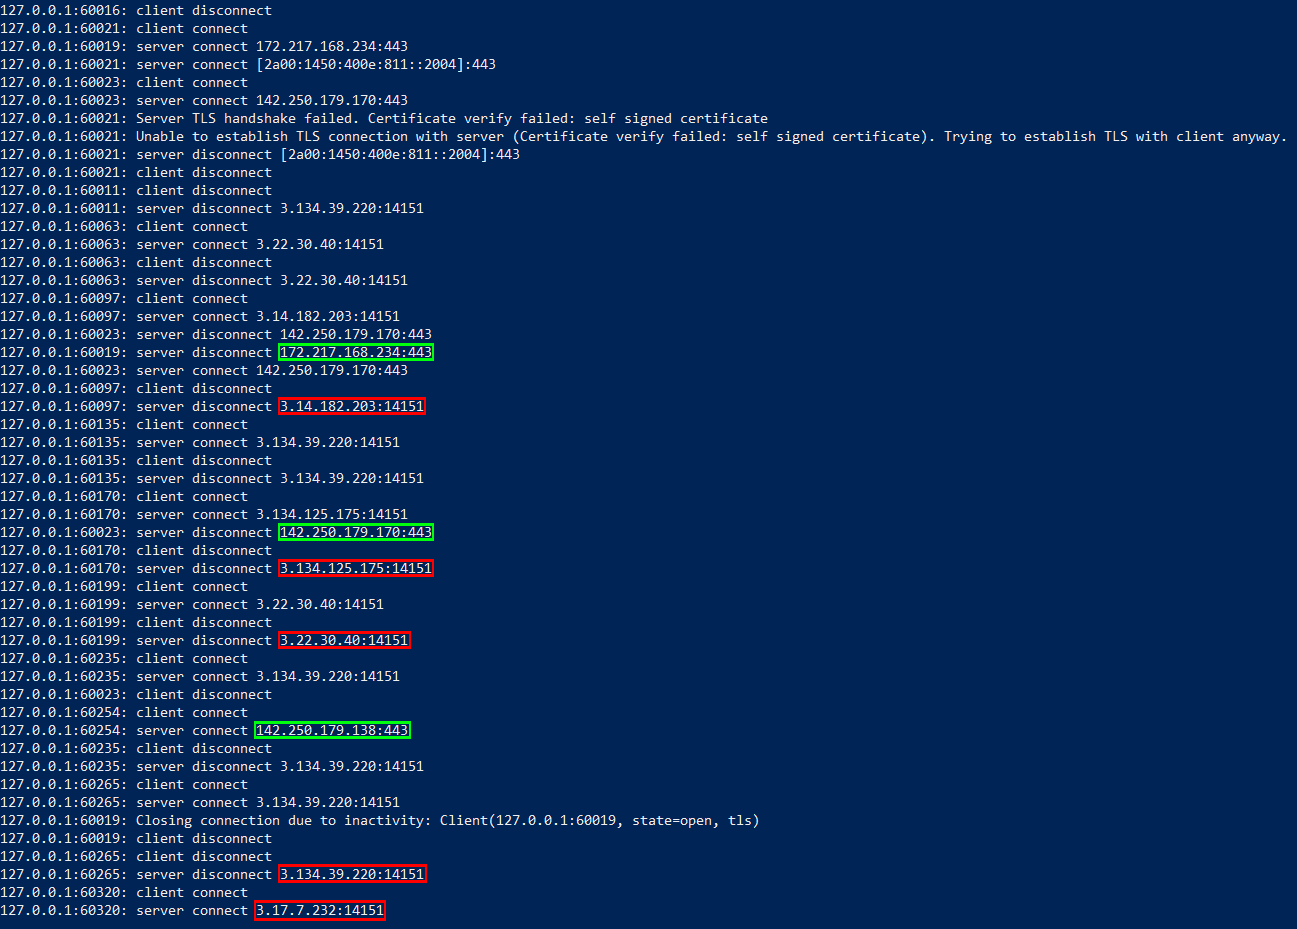
\includegraphics[width=0.85\textwidth]{MitmwebCapture.png}
    \caption{Captured network traffic with mitmproxy}
    \label{jordy-mitmweb}
\end{figure}

\newpage
\subsubsection{Wireshark analysis}
The captured network traffic in mitmproxy indicated that there were multiple connections to different IP addresses.
As described in subchapter 4.3.1 there was 1 range with 5 different IP addresses that kept looping.
The decision was made to focus on these 5 IP addresses since this range of IP’s were described on VirusTotal.
This was done with the following filter in Wireshark:

“(ip.addr == 3.22.30.40 || ip.addr == 3.17.7.232 || ip.addr == 3.134.125.175 || ip.addr == 3.134.39.220 || ip.addr == 3.14.182.203 || ip.src == 3.22.30.40 || ip.src == 3.17.7.232 || ip.src == 3.134.125.175 || ip.src == 3.134.39.220 || ip.src == 3.14.182.203)”.
 
The results of this filter are shown in the picture below.

\begin{figure}[H]
    \centering
    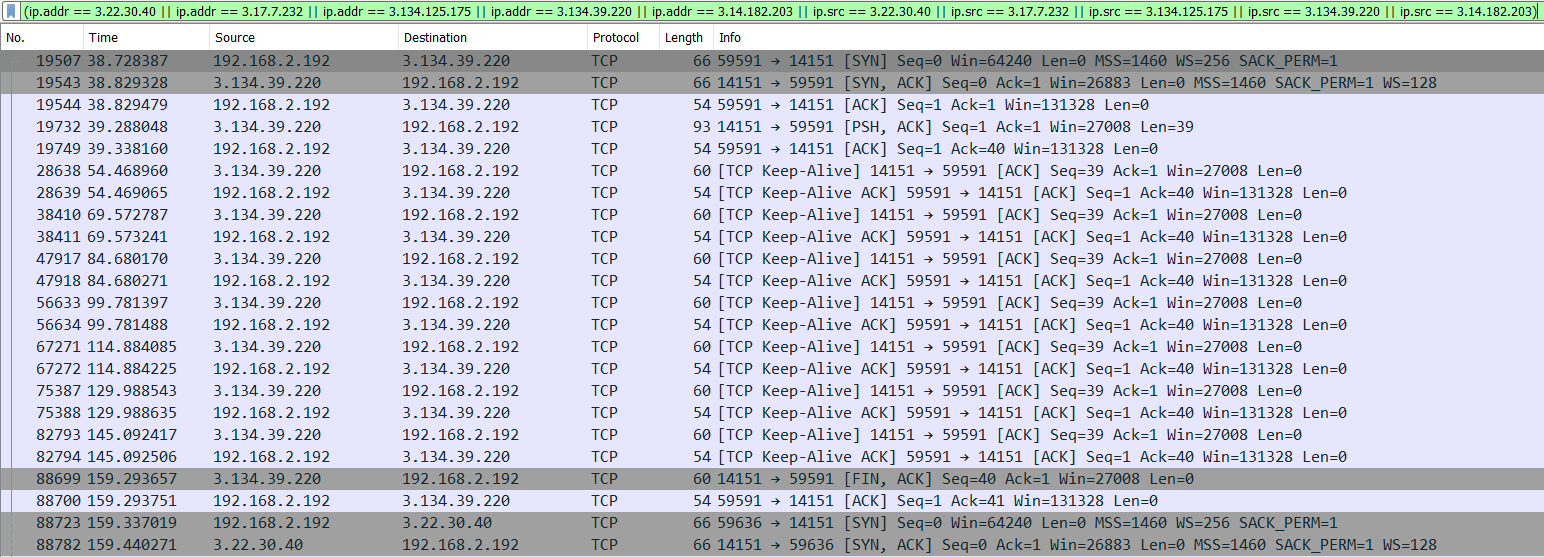
\includegraphics[width=1\textwidth]{WiresharkIPFilter.png}
    \caption{Captured network traffic with Wireshark filter specific IP's}
    \label{jordy-wiresharkfilter}
\end{figure}

Wireshark showed that the connection with different IP addresses all did the exact same thing.
The first grey line showed that the malicious application was asking to make a connection with the IP address.
The second grey line showed that the system on the IP address agreed to make a connection.
 
The first blue described that the two have made a connection.
The second blue line showed that the malicious application sends some data to the IP address.
From here on out it kept the connection alive till the IP address indicated that it wanted to terminate the connection with the third grey line.
From there it showed that both parties agreed to terminate the connection.
When the connection was terminated the application started the exact same process, but with a new IP address.

\newpage
It was not successful to try and determine exactly what data the application send over to the IP address that it made a connection with.
However it is likely that the application sends over information about the phone.

During the Wireshark analysis it was decided that it could be beneficial to look at the DNS traffic.
With the filter “DNS” in Wireshark all the DNS traffic on the laptop was captured.
When the application was installed on the phone one specific DNS stood out.
The specific DNS that stood out was “0.tcp.ngrok.io”.
This DNS was connected with one of the IP addresses that were found with mitmproxy.
The picture below shows the information in Wireshark.

\begin{figure}[H]
    \centering
    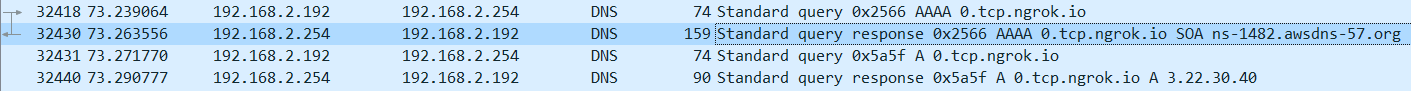
\includegraphics[width=1\textwidth]{WiresharkDNS Capture.png}
    \caption{Captured network traffic with Wireshark filter on DNS}
    \label{jordy-wiresharkDNS}
\end{figure}

It is very likely that behind the DNS “0.tcp.ngrock.io” a command and control server is hosted.

\subsubsection{Reconnaissance}

\href{https://www.shodan.io/host/3.14.182.203}{Shodan.io} was used to find out more about the different IP addresses.
All 5 of the IP addresses in the 3. range were owned by Amazon.
The location of the IP showed up as the city Hilliard in the United States and their server provider was Amazon.
It is likely that the people behind this application rent their servers from Amazon and when they have gotten enough complains or their scam is figured out they change the servers and IP’s that the application uses.
This would explain why the two described IP addresses on VirusTotal have not been seen during the network analysis.

The IP addresses in the 142. and 172. ranges were checked as well with \href{https://www.shodan.io/host/172.217.168.234}{Shodan.io}. It turned out that these IP addresses were owned by Google.
This meant that these IP addresses were not really interesting for the research.



\newpage
\subsection{Code analysis}
To get a better understanding of how the malicious application was build a code analysis was performed using jadx. The process and results of the code analysis are described in this chapter.

On first glance it became obvious that the people behind the application obfuscated the code. This meant that the code was difficult to understand. Because of this it was possible to get an idea of what the code did, but it was not possible to say with certain that it was correct.

In the code it was possible to confirm a lot of the permissions that were described in subchapter 4.1.2.1. Within the obfuscated code the following aspects of the application might have been traced:

\texttt{The application can read files.}
\newline \texttt{The application can read your contacts.}
\newline \texttt{The application can record your calls.}
\newline \texttt{The application can find your location.}
\newline \texttt{The application can record audio.}
\newline \texttt{The application can record video.}
\newline \texttt{The application can execute shell commands.}
\newline \texttt{The application can read SMS messages.}
\newline \texttt{The application can send SMS messages.}
\newline \texttt{The application can start up when the phone boots.}
\newline \texttt{The application can send information.}

In the code the word “keylogger” was present. This makes it very likely that the application contains a keylogger. The code for the keylogger has been described below:

\begin{figure}[H]
    \centering
    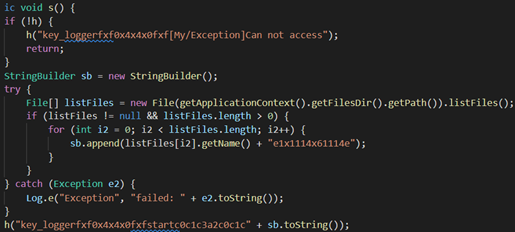
\includegraphics[width=1\textwidth]{CodeAnalysis2.png}
    \caption{Potential keylogger in the code}
    \label{jordy-keylogger}
\end{figure}

In the code there is a mention of an internet socket address. The code described below shows there is a high likelihood that the malicious application sends data through a network socket to the previously mentioned command and control server. 

\begin{figure}[H]
    \centering
    
\includegraphics[width=1\textwidth]{CodeAnalysis.png}
    \caption{Potential network socket in the code}
    \label{jordy-networksocket}
\end{figure}

\newpage
\subsection{Process analysis}
To get a better understanding of how the application affected the phone it was decided to preform a process analysis. The process and results are described in this chapter. 

To get a better understanding of how the malicious application affected the overall performance of the phone a process analysis was performed in Android studio. With the profiler in Android studio it was possible to check the CPU usage, memory usage and network usage. During the process analysis it became clear that the network and CPU usage stayed at 0 procent, however the memory usage kept slowly increasing over time. The two pictures described below were made at the startup and installation of the malicious applications and after an hour of running the application and showed the memory usage over time. 

\begin{figure}[H]
    \centering
    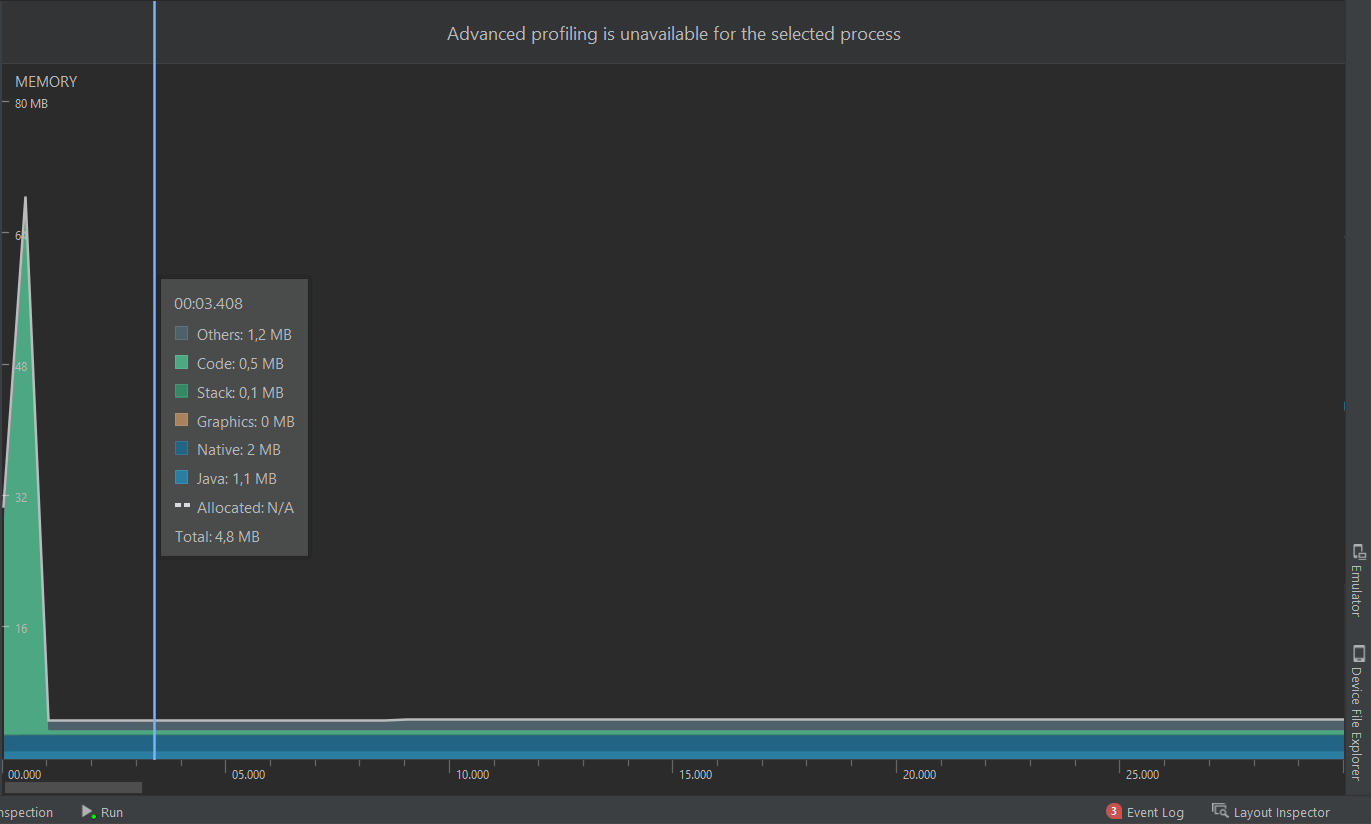
\includegraphics[width=1\textwidth]{MemoryStart.PNG}
    \caption{Memory on startup and installation of the application}
    \label{jordy-memorystartup}
\end{figure}

\begin{figure}[H]
    \centering
    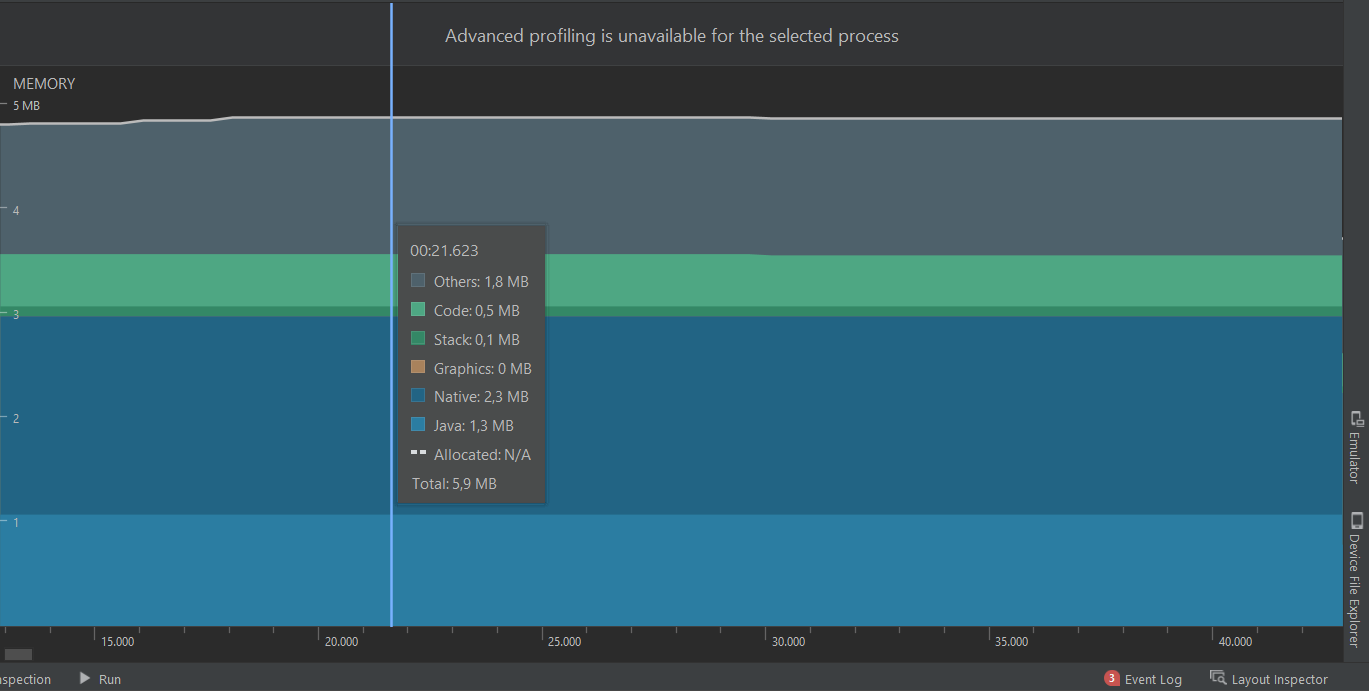
\includegraphics[width=1\textwidth]{MemoryEnd.PNG}
    \caption{Memory after an hour of running the application}
    \label{jordy-memory1hour}
\end{figure}

In the memory usage it was shown that the memory being used very slowly increased. The areas that the memory usage increased in were the others, native and java areas. This did not give any more information about why the memory usage slowly increased but it was interesting to see.

\newpage
\subsection{Countermeasures and detection}
A part of malware analysis is coming up with countermeasures and ways to detect the application.
The different countermeasures are described in this chapter.

\subsubsection{Preventive measures}
There would be a few preventive measures to not install this malicious application.
One of these was to only install applications that are on the official Google Play Store.
The only Firefox application that is downloadable on the Google Play Store is the official application from Mozilla.
This would mean that the malicious application is not able to be installed on an user’s phone.

The other preventive measure was to install an antivirus software on the user’s phone.
The antivirus software would flag the malicious application as malware and would give a notification or block the installation all together.

\subsubsection{Detective measures}
The best way to detect that the malicious application was installed was by checking the notification bar.
The application always showed up in the notification bar as “FireFox” with “Browser” underneath it.
When this notification was clicked it showed nothing.

Another way to detect the malicious application is by looking in the settings app and checking the apps tab.
In this part of settings all installed apps are shown.
The malicious application said it was not installed but showed up in this list.
This meant that the application was indeed installed.

The last described detective measure is installing an antivirus software.
Many security vendors including AVG AntiVirus showed on VirusTotal that the application was malicious.
The antivirus software would indicate that the application is malicious and would give the user a warning.

\subsubsection{Reactive measures}
When the application is detected on a device it is important to immediately uninstall the application.
With the permissions the application asks for it is possible that it send a lot of information to the command and control server and it could do a lot of damage to the Android installation on the phone.
Since the malicious application has the permission to install packages it would be advised to check all installed apps and uninstall any apps the user does not know.
The best solution would be to do a factory reset of the phone.

\subsubsection{YARA rule set}
A YARA rule set is intended to automatically find a specific group of applications.
The designed YARA ruleset that is shown below is designed to specifically find this malicious application using the start of the classes.dex hex code.

\lstinputlisting[language=YARA]{individual/jordy/ruleset.yara}

\newpage
\section{Doodle Jump 2 Application Analysis by Michael}

The following research has been done for the video game application ‘Doodle Jump 2’, downloaded from the Google Play Store. The package name of the official version is ‘com.limasky.doodlejump2’. The malicious version of this game was downloaded from Koodous. The version of the app that has been researched is 1.4.7. Remarkably, the legitimate version of this application is smaller than the malicious version. The real APK being 47,8MB in size and the modified APK being 36,47MB.
\subsection{VirusTotal summary}


\noindent\makebox[\textwidth]{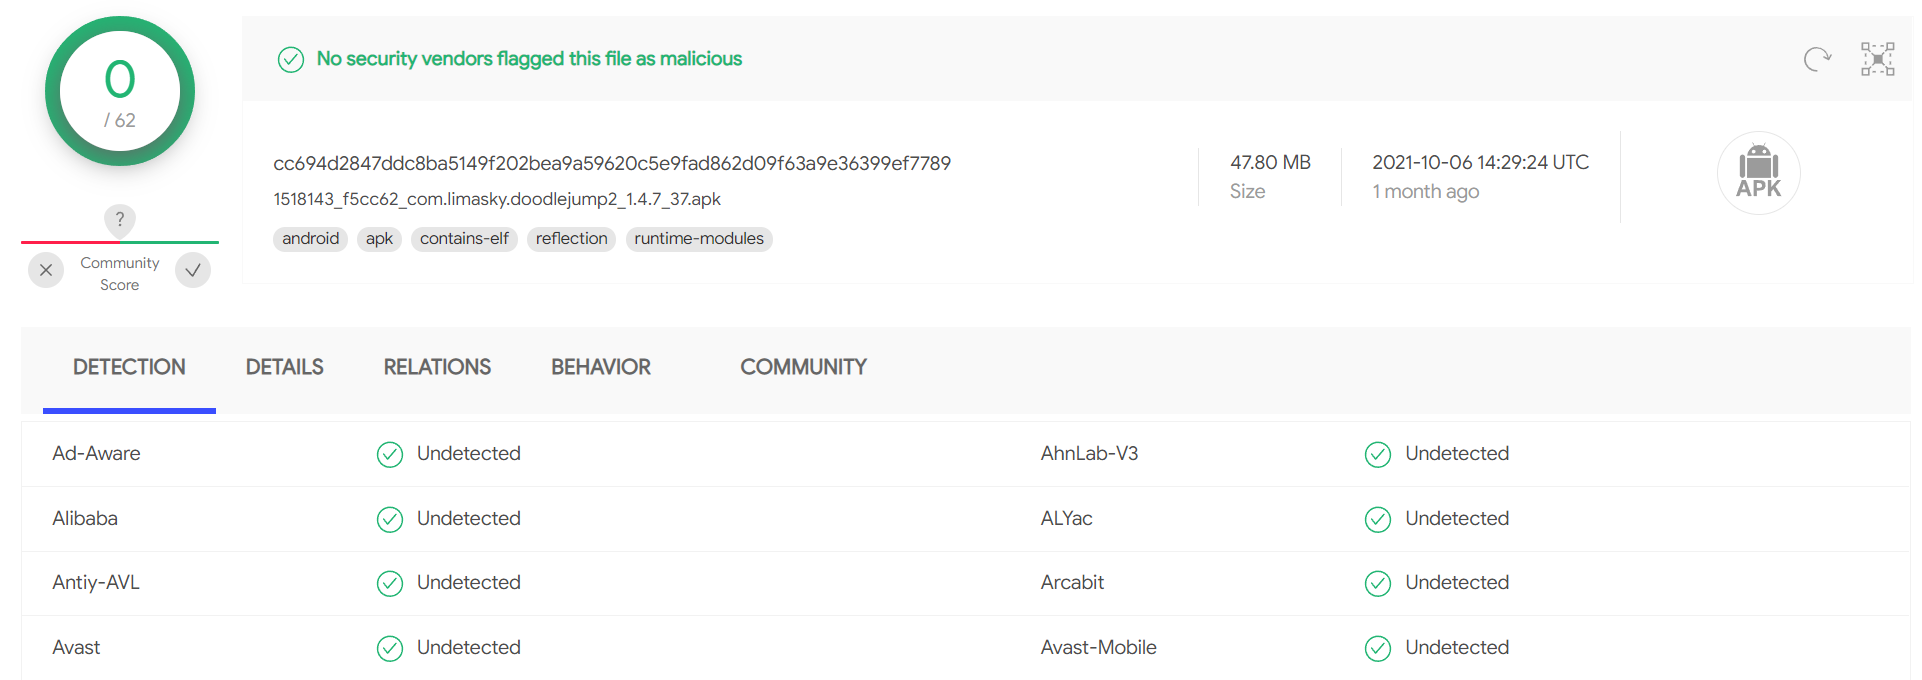
\includegraphics[width=\textwidth]{michael1.png}}

As can be seen in the above screenshot, Virustotal does not detect any kind of malicious content for the version that has been downloaded from the Google Play Store. Since this is a relatively popular app on the Google Play Store, with over 500 thousand downloads, it is safe to assume that these measurements are accurate.

\noindent\makebox[\textwidth]{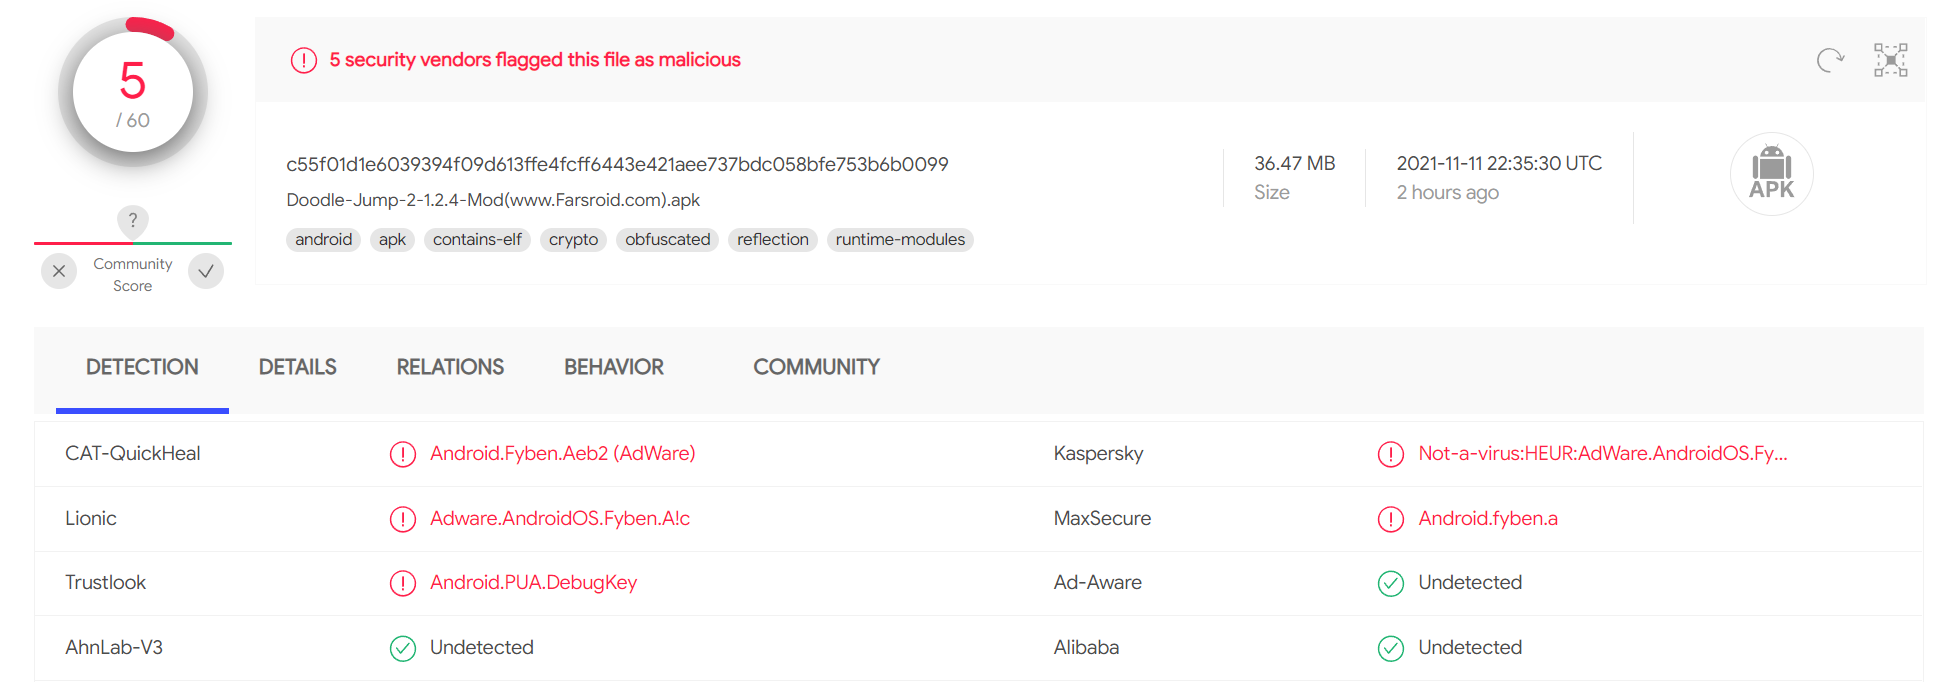
\includegraphics[width=\textwidth]{michael2.png}}

As for the Doodle Jump 2 application that I have found on Koodous, it seems this one is far more malicious than the one found on the app store. In the above screenshot it has been made clear that VirusTotal has found several issues. This APK file contains AdWare. AdWare is unwanted software that spams the user with a lot of advertisements on the screen. The attacker usually profits off of this by monetary gain. Obviously, none of the hashes match with the original version.
\subsubsection{Permission requests}

%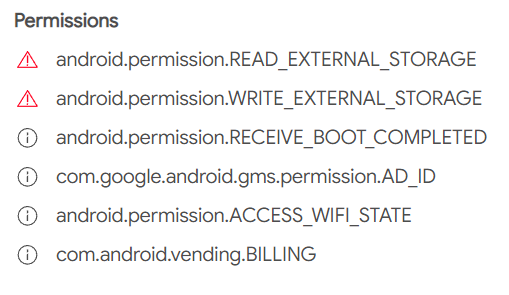
\includegraphics{michael3.png}
\begin{minipage}{\linewidth}
\begin{wrapfigure}{r}{0.5\textwidth}
\centering
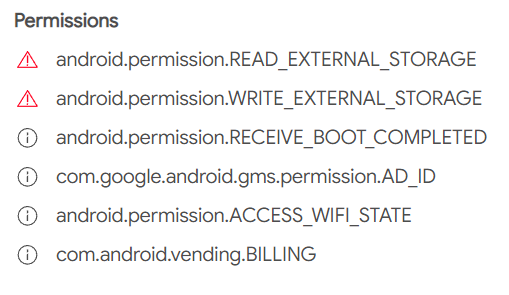
\includegraphics[scale=0.35]{michael3.png}
\end{wrapfigure}

~\\
~\\
The permissions this app requires are reasonable for a game. Reading and writing to external storage might be useful for future updates, so despite the warnings, it is still safe to assume that the app is not malicious.
\end{minipage}

~\\
~\\
~\\
~\\
~\\
~\\

%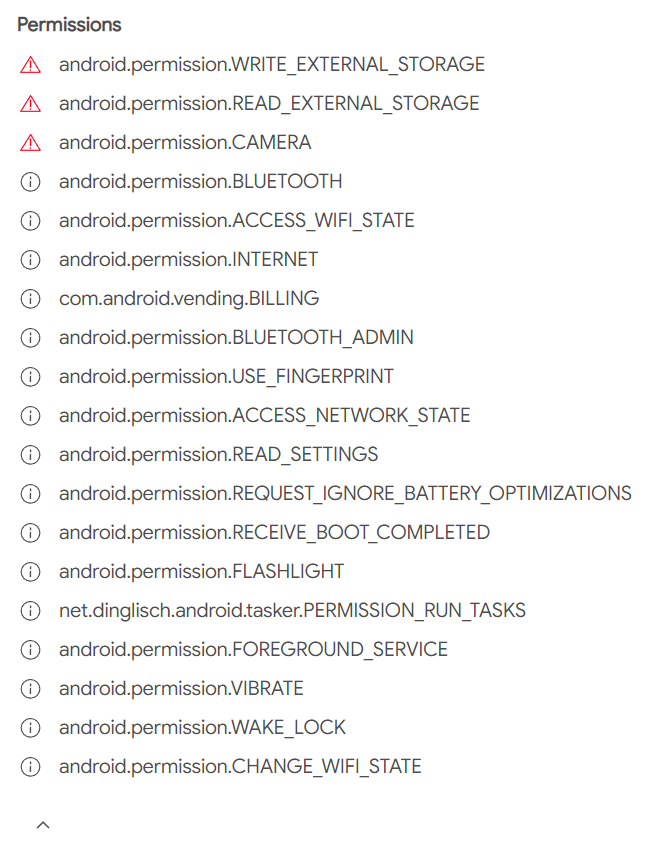
\includegraphics{michael4.png}
\begin{minipage}{\linewidth}
\begin{wrapfigure}{l}{0.55\textwidth}
\centering
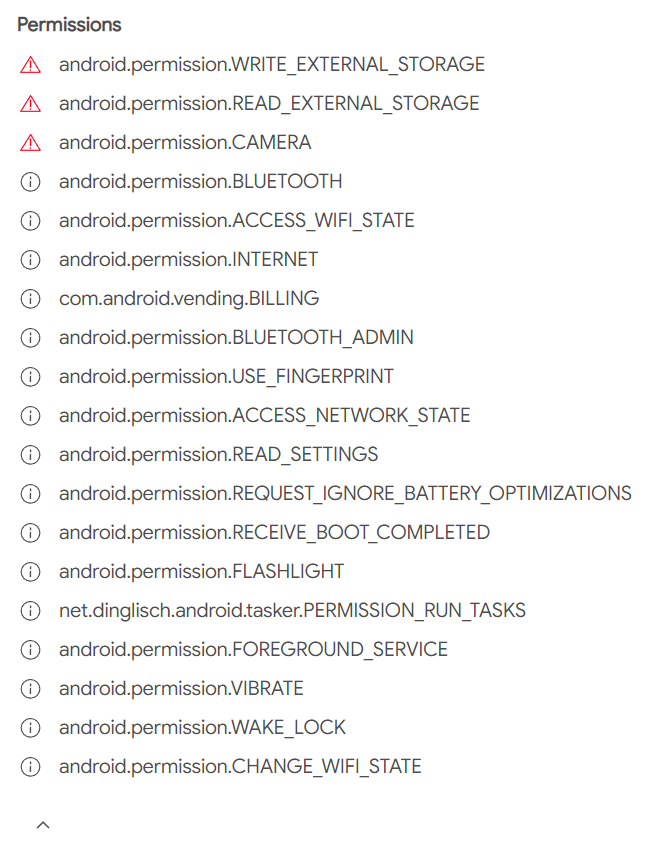
\includegraphics[scale=0.3]{michael4.png}
\end{wrapfigure}

~\\
~\\
As can be seen, a lot more permissions are required than from the official version. What these permissions are for can be read, but what they are actually being used for is unknown. Most likely for malicious activity.

\end{minipage}

\newpage
\subsection{Behavior analysis}


%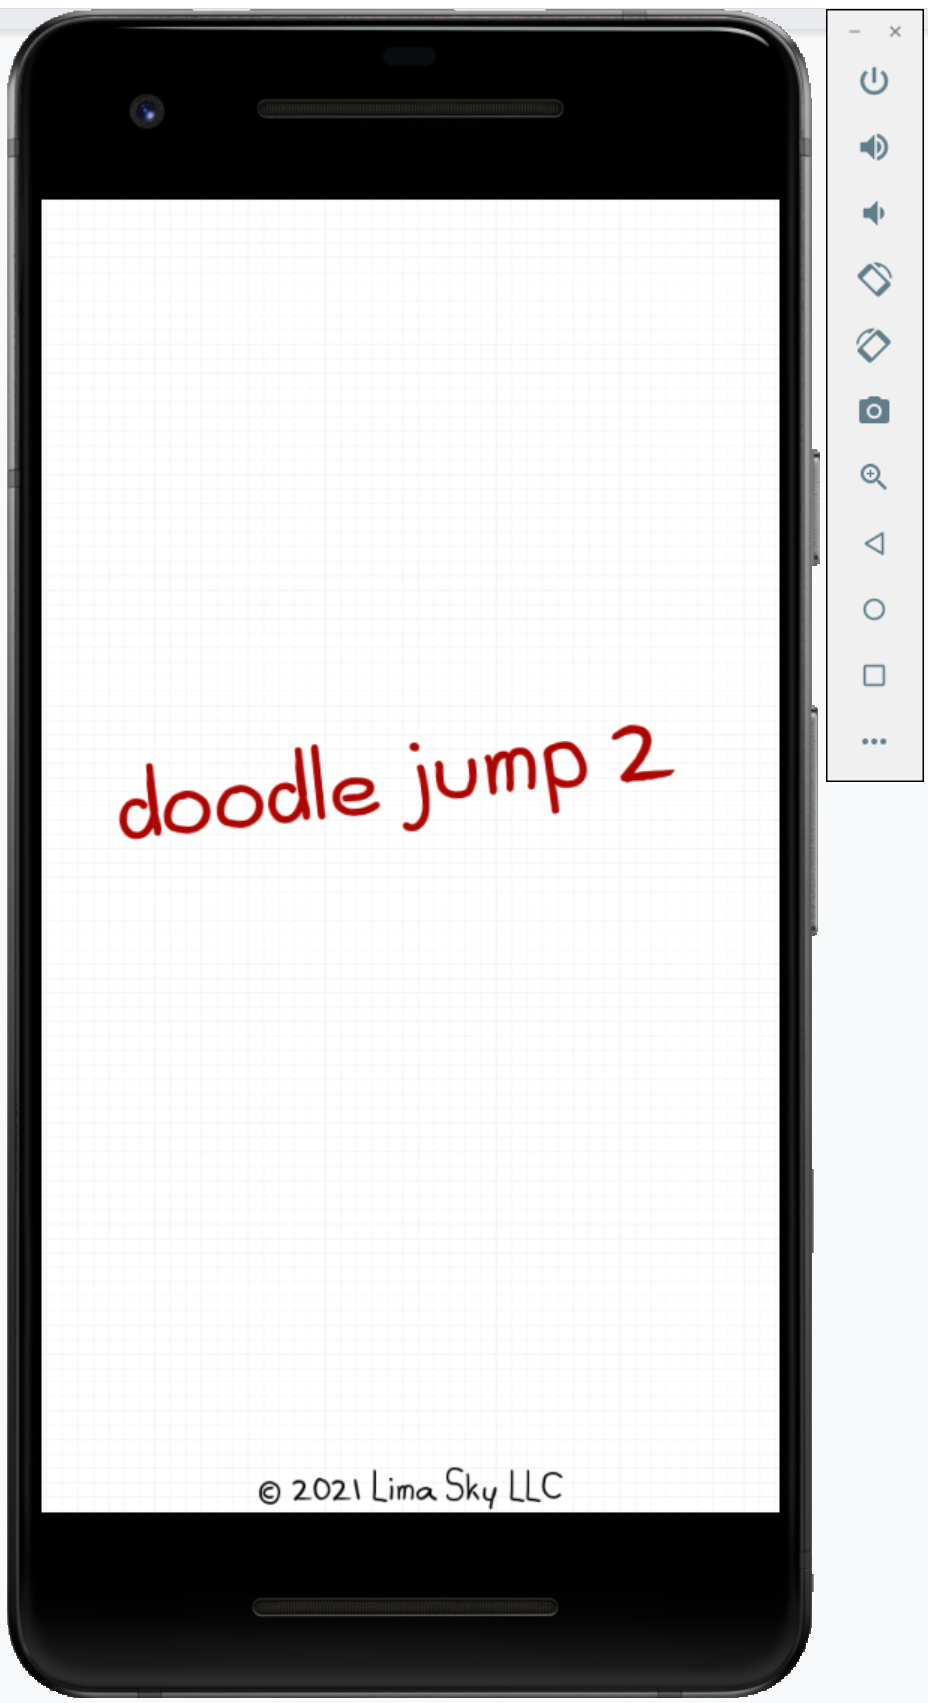
\includegraphics[width=4cm]{michael5.png}

\begin{minipage}{\linewidth}
\begin{wrapfigure}{l}{0.4\textwidth}
\centering
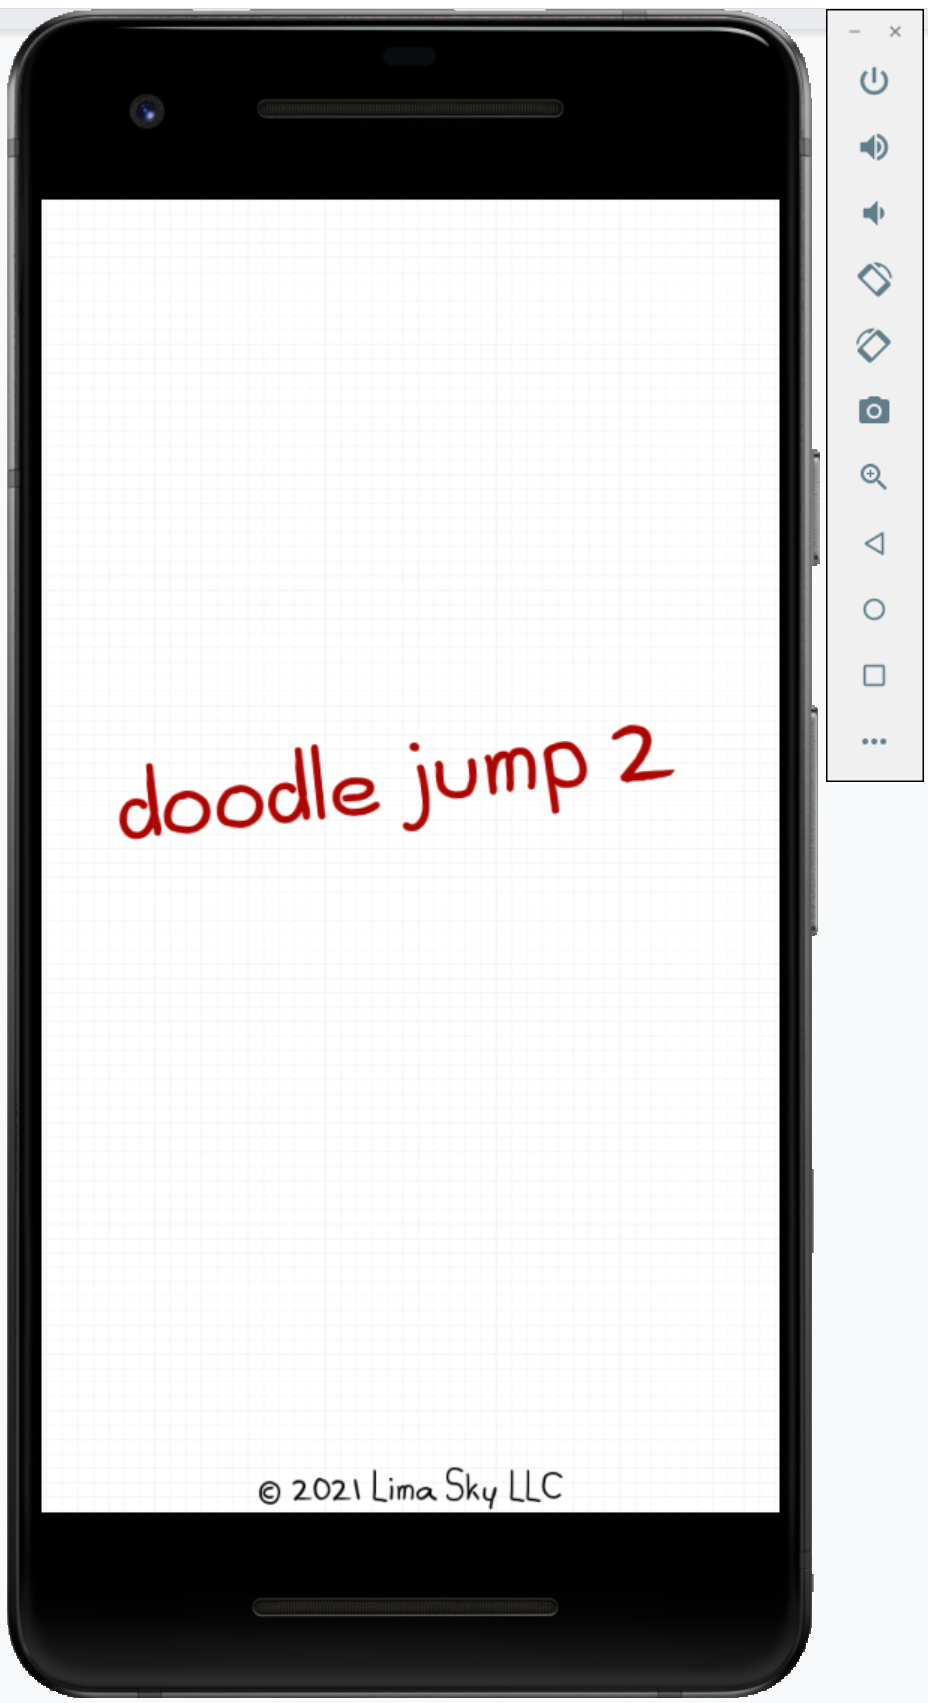
\includegraphics[scale=0.15]{michael5.png}
\end{wrapfigure}

~\\
~\\
During the installation process and gameplay of the original application, nothing out of the ordinary was found. After the installation was done the application could be found in the app drawer with its corresponding icon. Booting up the application everything worked fine. The screen, which can be seen in the screenshot above, was shown. After that it was possible to play the game starting from level one. Since this game requires tilting, it was hard to actually progress in the levels, but still it worked to some degree which made it certain that the game was running as it should.

\end{minipage}

~\\
~\\
~\\
~\\
~\\
~\\
~\\
~\\
~\\
~\\
~\\
~\\
~\\
~\\
~\\
~\\
~\\
~\\
~\\
~\\
~\\
~\\
~\\
~\\
~\\
~\\
~\\

\newpage

\begin{figure}
\centering
\begin{minipage}{.5\textwidth}
  \centering
  
\includegraphics[width=.4\linewidth]{michael6.png}
  \caption{Legitimate Application}
  \label{fig:test1}
\end{minipage}%
\begin{minipage}{.5\textwidth}
  \centering
  
\includegraphics[width=.4\linewidth]{michael7.png}
  \caption{Malicious Application}
  \label{fig:test2}
\end{minipage}
\end{figure}

As for the malware-ridden application, the installation also went smoothly. It was however necessary to uninstall the previous application, since Android thought this app to be a downgraded version of the previous one. After uninstalling the other app this one worked fine. Nothing seemed out of the ordinary until the app had actually been installed. Namely, the app icon in the app drawer for the game did not seem to match entirely with that of the original app. It is similar, however, it seems like it has been zoomed out a bit. See above for comparisons.

%
\includegraphics[width=4cm]{michael8.png}
\begin{minipage}{\linewidth}
\begin{wrapfigure}{l}{0.4\textwidth}
\centering

\includegraphics[scale=0.15]{michael8.png}
\end{wrapfigure}


Attempting to run the app, the user is greeted with some kind of Arabic message. The most interesting part in this message was perhaps a link to an url. It leads to a website which is also entirely in Arabic. A lot more applications could be found on this website, even some of the more known ones. It seems like the website of a hobbyist who likes to distribute modified versions of Play Store applications. Tapping either ‘Don’t show again’ or ‘OK’ on the message allows the user to get in the application, and it continues booting up like normal.\\
The first thing anyone would notice when attempting to play the game is that all the levels are unlocked from the start with extremely high scores. All in-game achievements have been cleared too, in this case stars. This seems strange, since it does not incentivize players to actually play the game. What is even more interesting is that when a player would select a level to play, the character immediately falls at a score of 21. This happens at every level. The game is thus impossible to play. The entire application or phone also feels much slower, however, a memory analysis would have to be performed to confirm this hypothesis. Shutting down the app does not cause any issue, and it is possible to boot up the application again. After rebooting the game and performing a couple more tests, it seemed like the game was finally playable. The app ran at a decent speed, and it was possible to play the levels without immediately dying. It also seemed like the player earned a higher score more quickly. Despite adware being reported in VirusTotal, other than the message when booting up, no other ads or pop ups have been found.

\end{minipage}

\newpage
\subsection{Network analysis}

\begin{center}
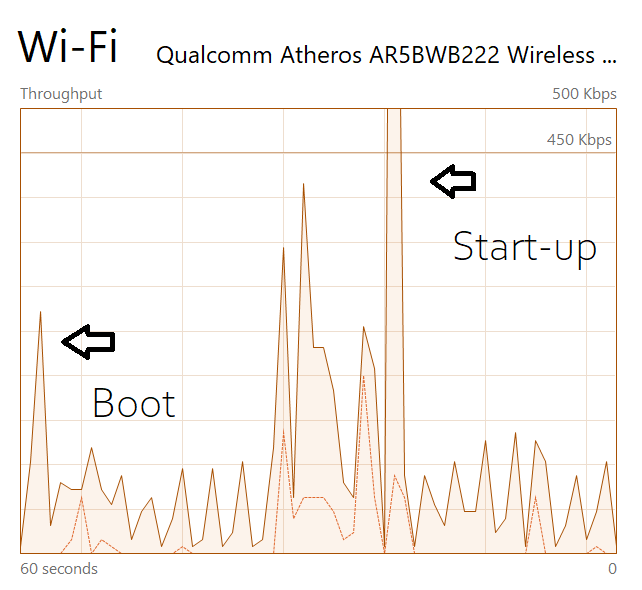
\includegraphics[scale=0.5]{michael9.png}
\end{center}

Since the graph for both the malicious, as well as the legitimate application both look the same, only one of them will be displayed. When booting up the application, there was a small spike of network usage. A possibility might be that this was when the application is connecting with the server to look for updates. This would have to be confirmed during the code analysis.
After booting up it takes a small amount of time for the application to load, after which there is a huge network spike. What this is for is as of yet unknown, but an educated guess would be to load scores for levels. Also this would have to be confirmed during the code analysis.
\subsubsection{HTTP proxy analysis}
The two captures that have been made were done so after the app was booted and initialized. The first one is for the legitimate application and the second one is for the malicious application. At first glance they don’t seem different from each other, however there are some inconsistencies.

\noindent{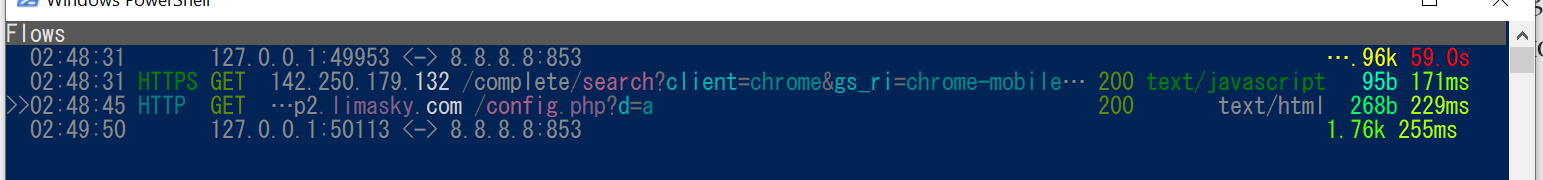
\includegraphics[width=\textwidth]{michael10.png}

The above screenshot was the output of mitmproxy for the legitimate application. Nothing seems out of the ordinary. There was a GET request for google, most likely an Android service in the background. Other than that there was a GET request for a config.php file towards the Limasky servers, which are the developers of the app. This one was not encrypted, it was a simple HTTP request. The contents, however, are not interesting.

\noindent{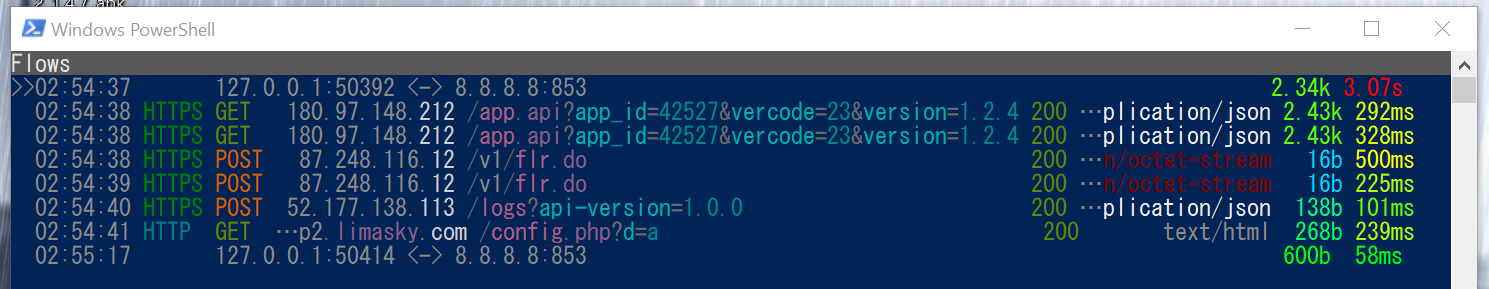
\includegraphics[width=\textwidth]{michael11.png}

This capture seems to have two GET requests and three POST requests that have to do with some kind of API. The three IP addresses associated with these requests are from huge internet companies, such as Microsoft Azure and Yahoo! UK. From this it is clear that these are thus not relevant, and are the result of a background process. Other than that, the same GET request to the Limasky servers had been made.
\subsubsection{Wireshark analysis}

\noindent{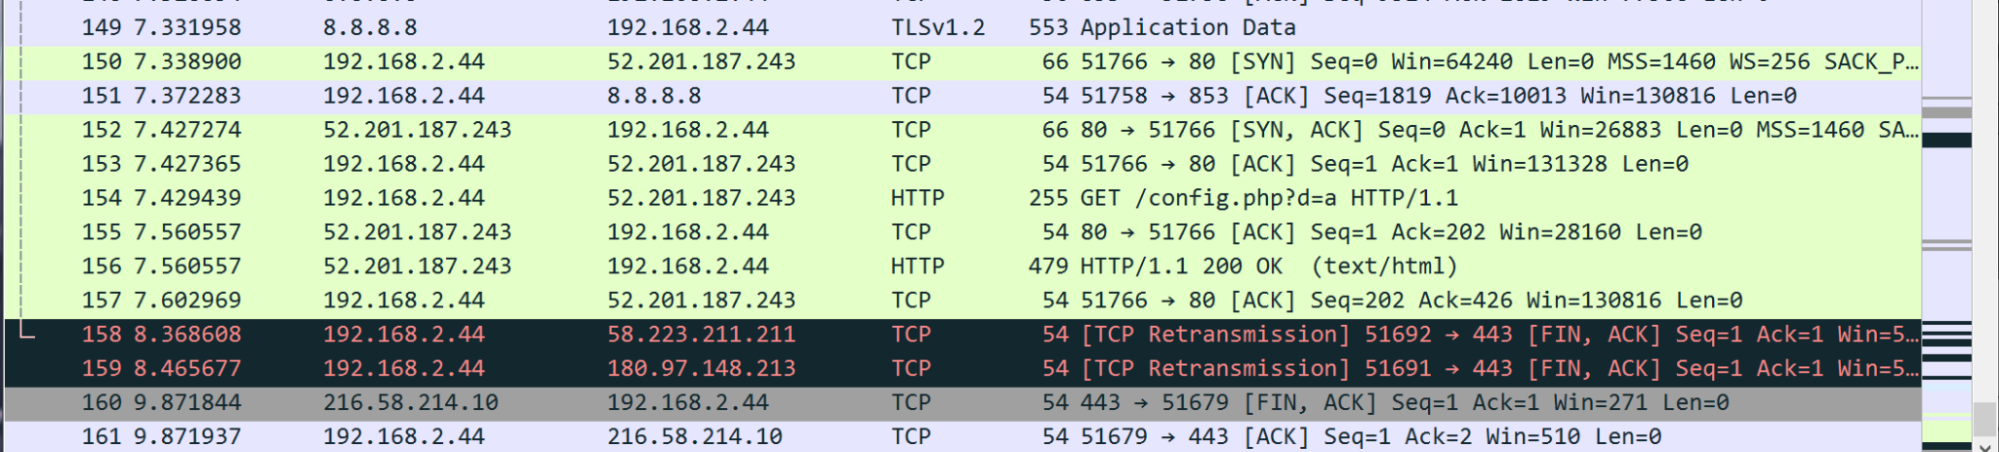
\includegraphics[width=\textwidth]{michael12.png}

For the Wireshark analysis, the malicious app was tested first. Interestingly, during start-up a TCP handshake was being performed. Other than this data there is nothing else that might be relevant. A scan has been performed on the IP address, and from this scan it became apparent that the IP is hosted by Amazon Web Services in the United States of America. This was surprising, considering malicious activity more than likely gets removed sooner or later from big hosting companies such as these. However, what happened next would subdue all suspicion one could have.

\noindent{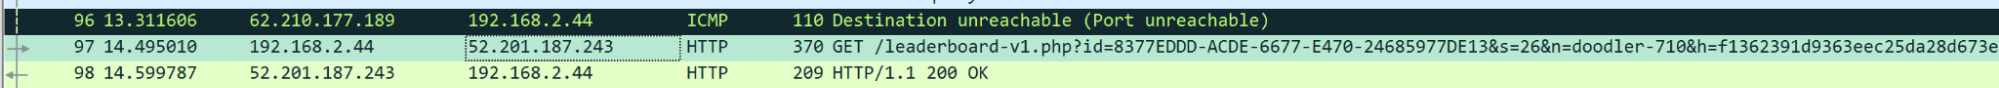
\includegraphics[width=\textwidth]{michael13.png}

The application was allowed to continue to run, and when this happened, a GET request was made to the exact same IP as before. This could only mean that this packet could only go to the legitimate source of the application. This is disappointing, but enlightening at the same time, since it is now clear that this application is not being used for harmful or malicious purposes. To confirm this hypothesis, the legitimate application was executed and tested with Wireshark and showed the exact same output as the malicious version. This means there is no malicious network traffic being found. This analysis does confirm what happened during the general network analysis, that for both applications the same amount of network traffic is being transmitted.
\subsubsection{Reconnaissance}

Using shodan.io, much of the information on the network analysis part of the research could be found. For the IP’s that had significance, shodan.io was used. This way it was also possible to identify what kind of hard services were provided on those networks, which in turn cleared up the picture as for what these connections were used for.

\newpage
\subsection{Code analysis}
To analyze the code of the applications, it was necessary to decompile them using a program called JadX. After this was done, Dex2Jar was used to confirm the process was completed successfully.

%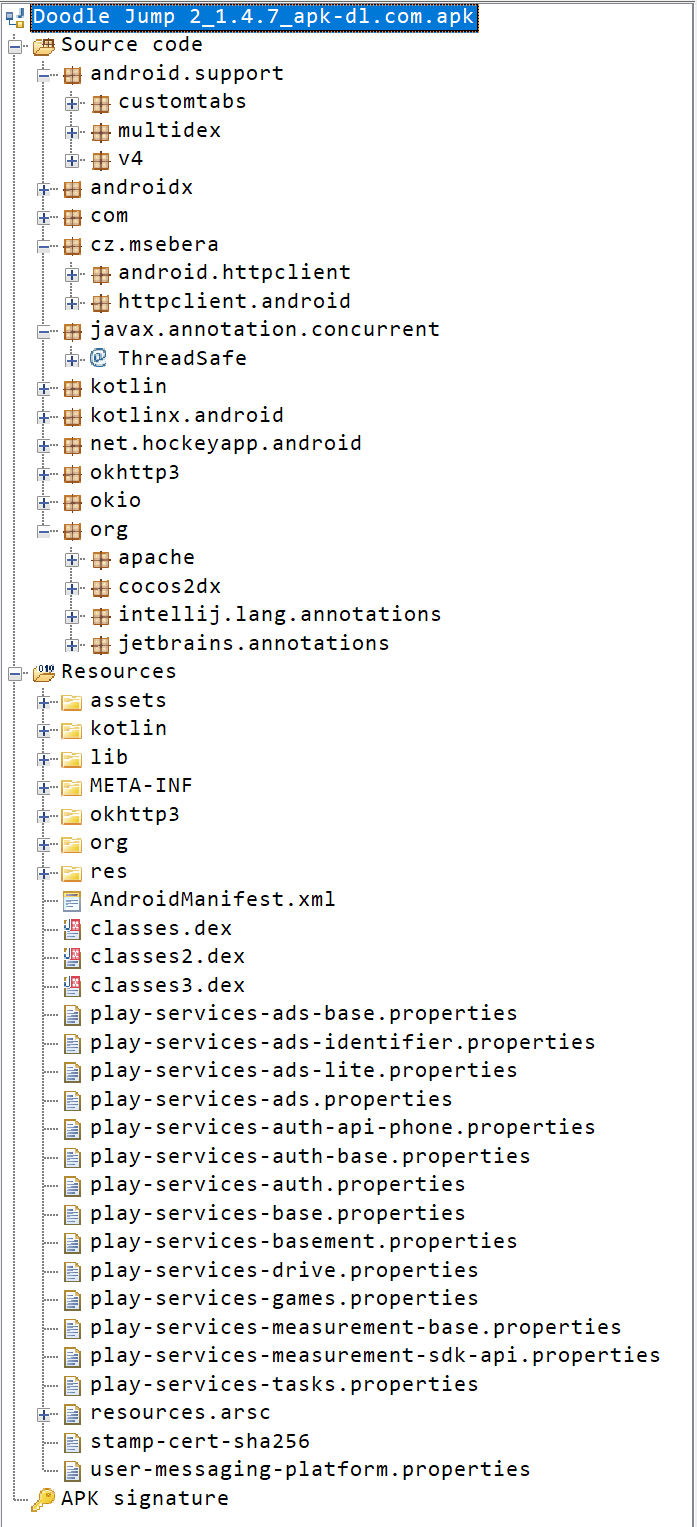
\includegraphics[width=4cm]{michael14.png}
%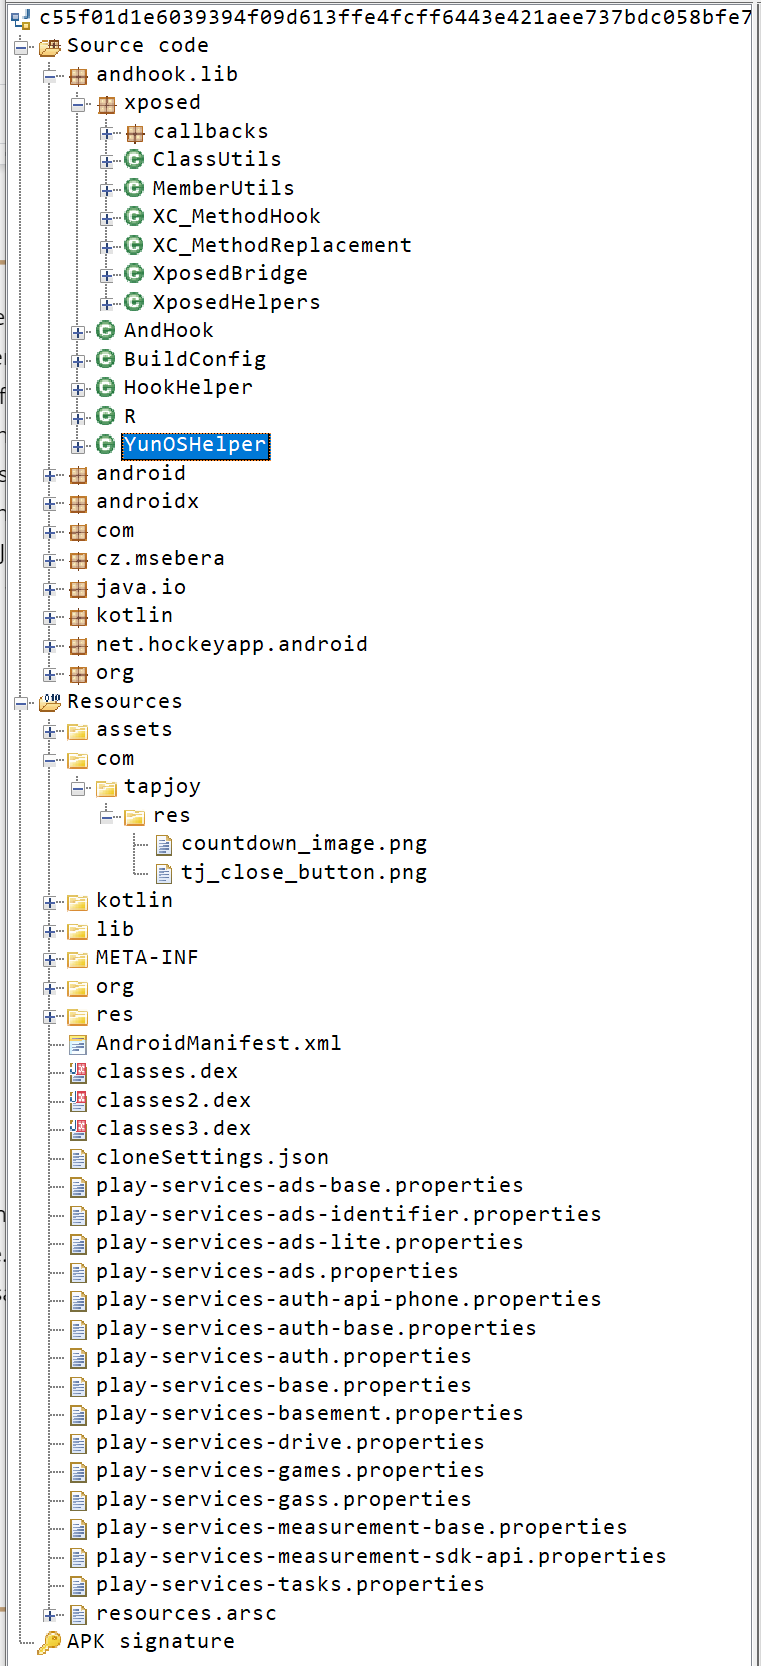
\includegraphics[width=4cm]{michael15.png}

\begin{figure}
\centering
\begin{minipage}{.5\textwidth}
  \centering
  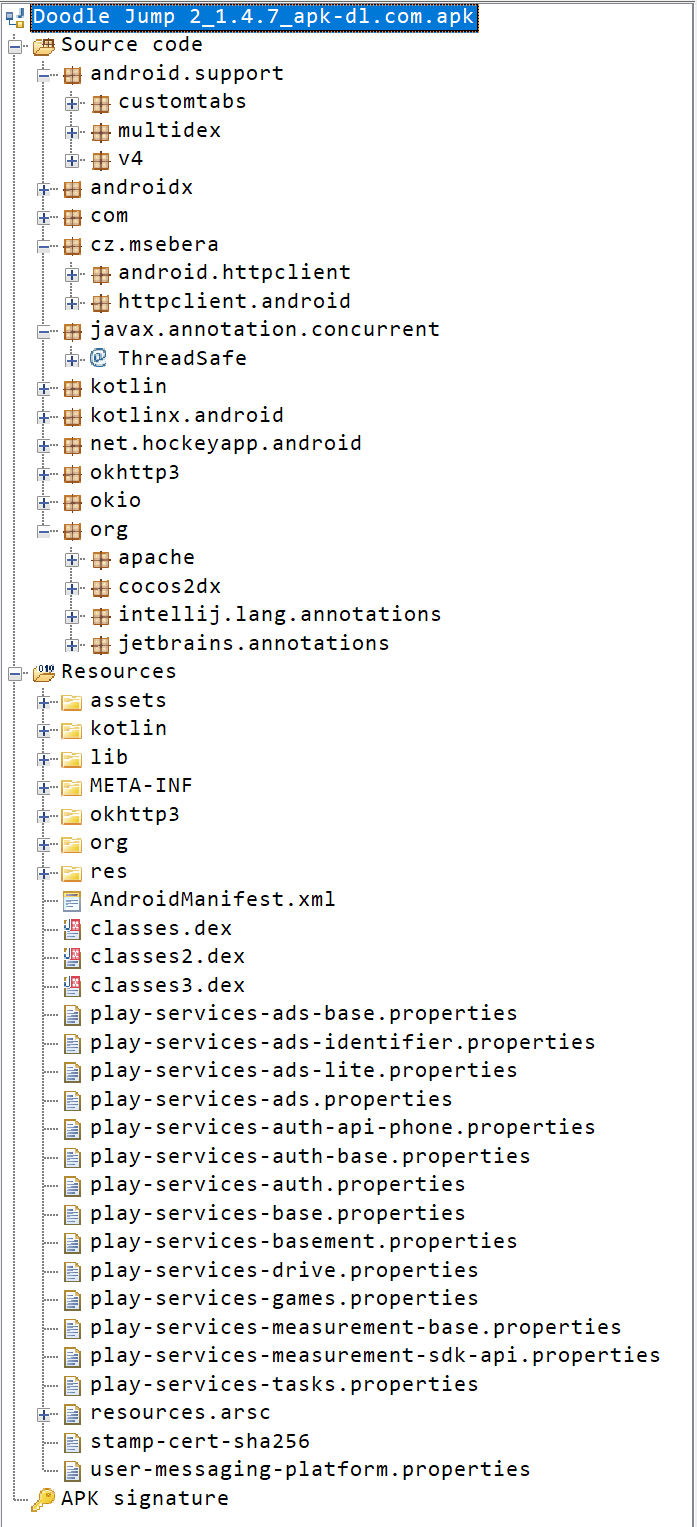
\includegraphics[width=.6\linewidth]{michael14.png}
  \caption{Legitimate Application}
  \label{fig:test1}
\end{minipage}%
\begin{minipage}{.5\textwidth}
  \centering
  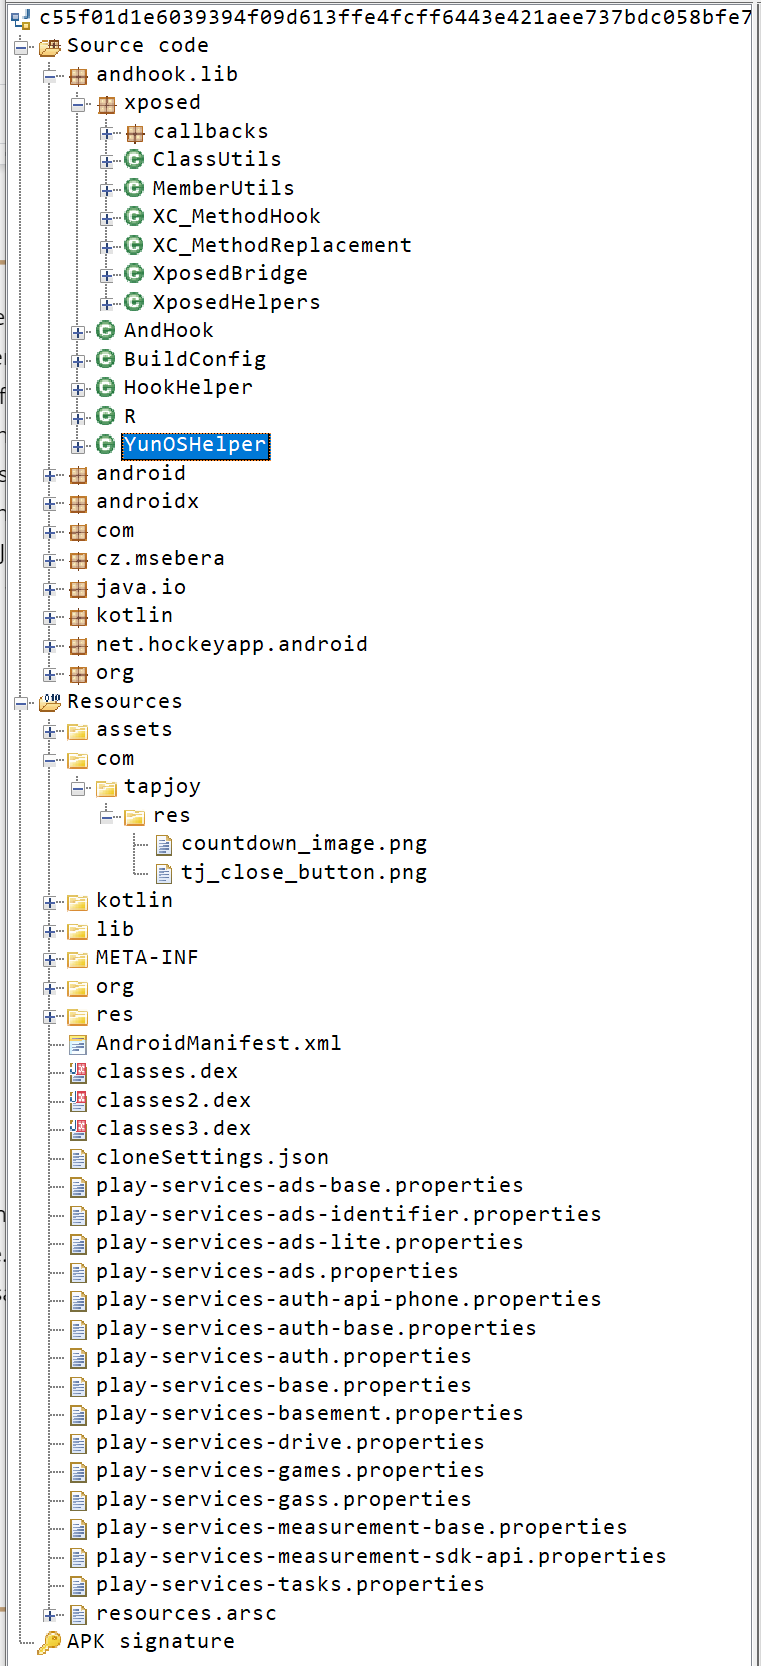
\includegraphics[width=.6\linewidth]{michael15.png}
  \caption{Malicious Application}
  \label{fig:test2}
\end{minipage}
\end{figure}

As for the source code, nothing out of the ordinary has been found. After going through the folders the usual files and folders to be included for a video game, such as a MathKt class and assets folder, were present. It is also safe to assume that the application has been written in Java on the IntelliJ IDEA development environment by JetBrains, since there were packages for development on that editor.

For the malicious version, the first thing anyone would notice is the absence of a couple of folders compared to the legitimate application, and the presence of new ones. There is now an andhook.lib library in the source code. What this does is not entirely clear and requires a higher level of understanding of game programming. Another folder I have noticed appearing is the ‘com’ folder in resources. This folder contains an image for some kind of countdown, and another for a close button. Since AdWare has been found, one would assume that these images are being used for pop-up ads which users are able to close once the countdown is over. However, during the behavior analysis, no such behaviour has been detected.

\newpage
\subsection{Process analysis}
For the memory analysis, a reliable tool, named Simple System Monitor was used. This is a popular app on the Play Store to track the usage of the CPU and RAM. However, the CPU details could not be recorded since the device is emulated. This is highly unfortunate, but at least it is possible to note the RAM usage.

%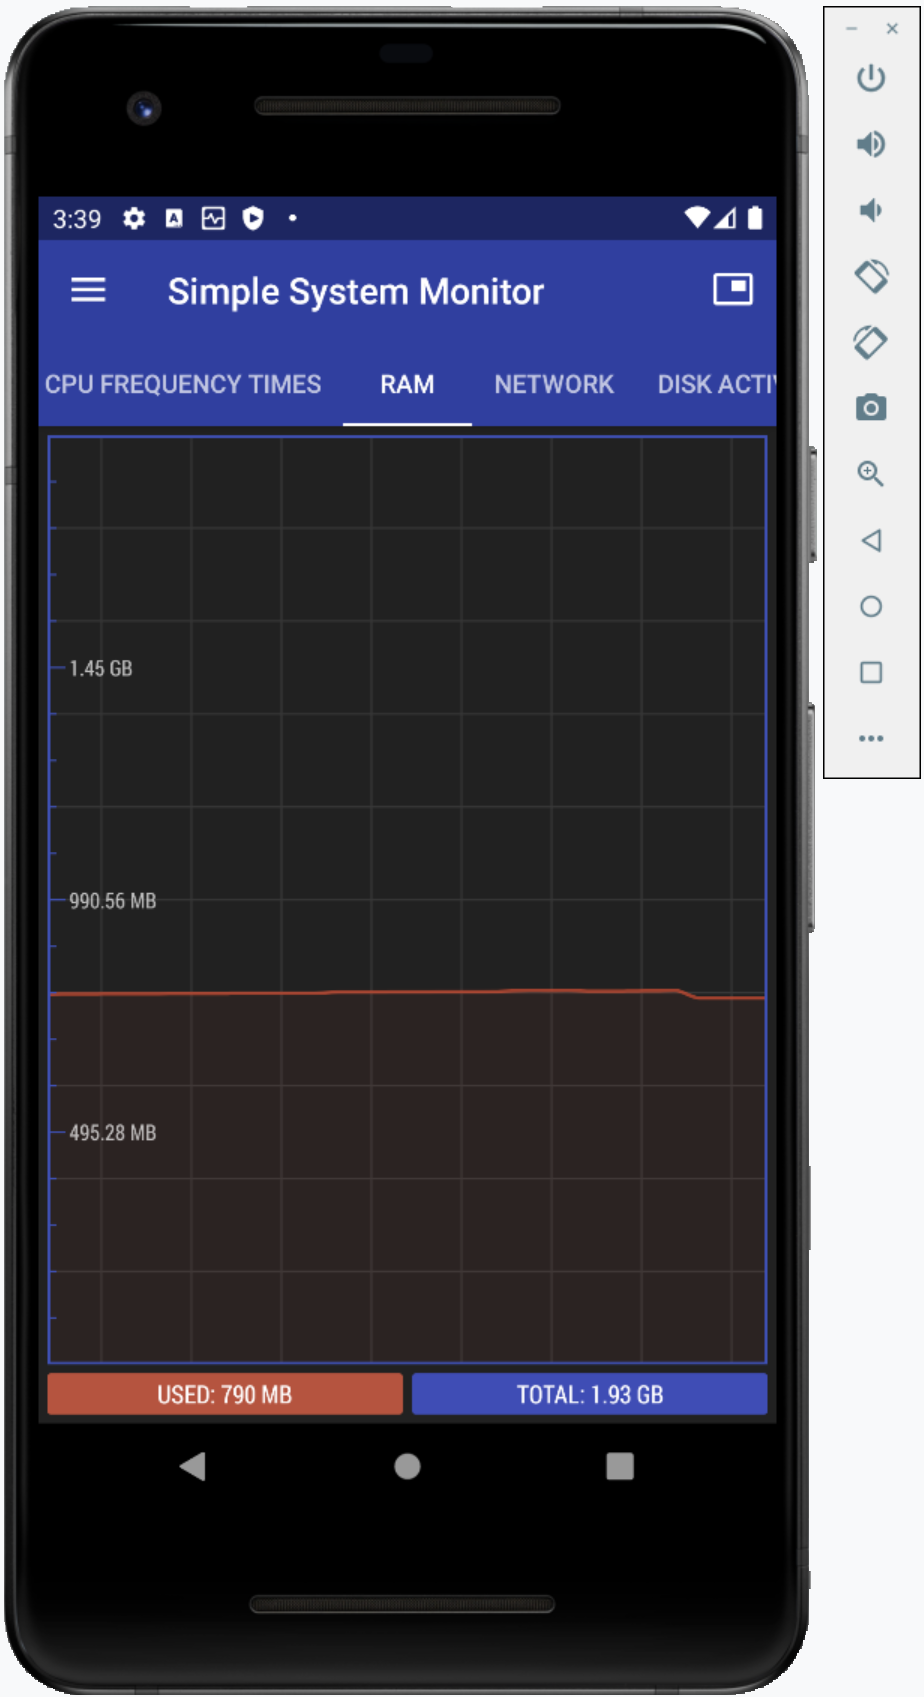
\includegraphics[width=4cm]{michael16.png}
\begin{minipage}{\linewidth}
\begin{wrapfigure}{l}{0.4\textwidth}
\centering
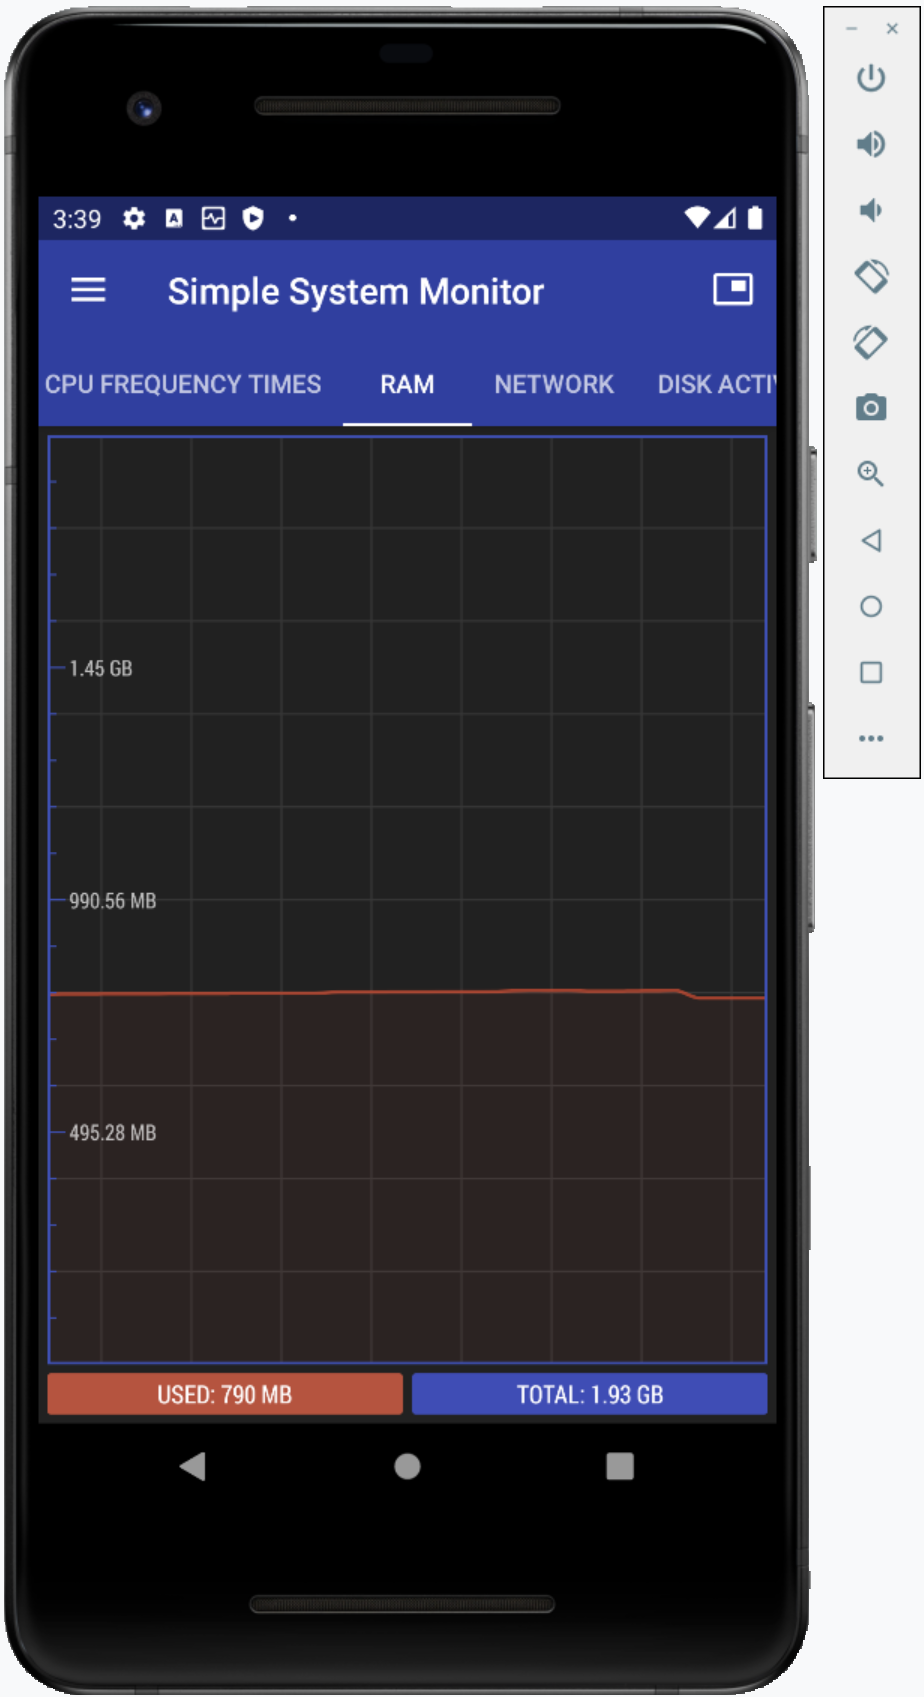
\includegraphics[scale=0.15]{michael16.png}
\end{wrapfigure}
~\\
~\\
~\\
~\\
~\\
~\\
~\\

This was the RAM usage while idle. As can be seen, it consists of a stable 790MB of data used. This was most likely being used by native Android processes, since no other processes are currently running.
\end{minipage}
~\\
~\\
~\\
~\\
~\\
~\\
~\\
~\\
~\\
~\\
~\\
~\\
~\\

%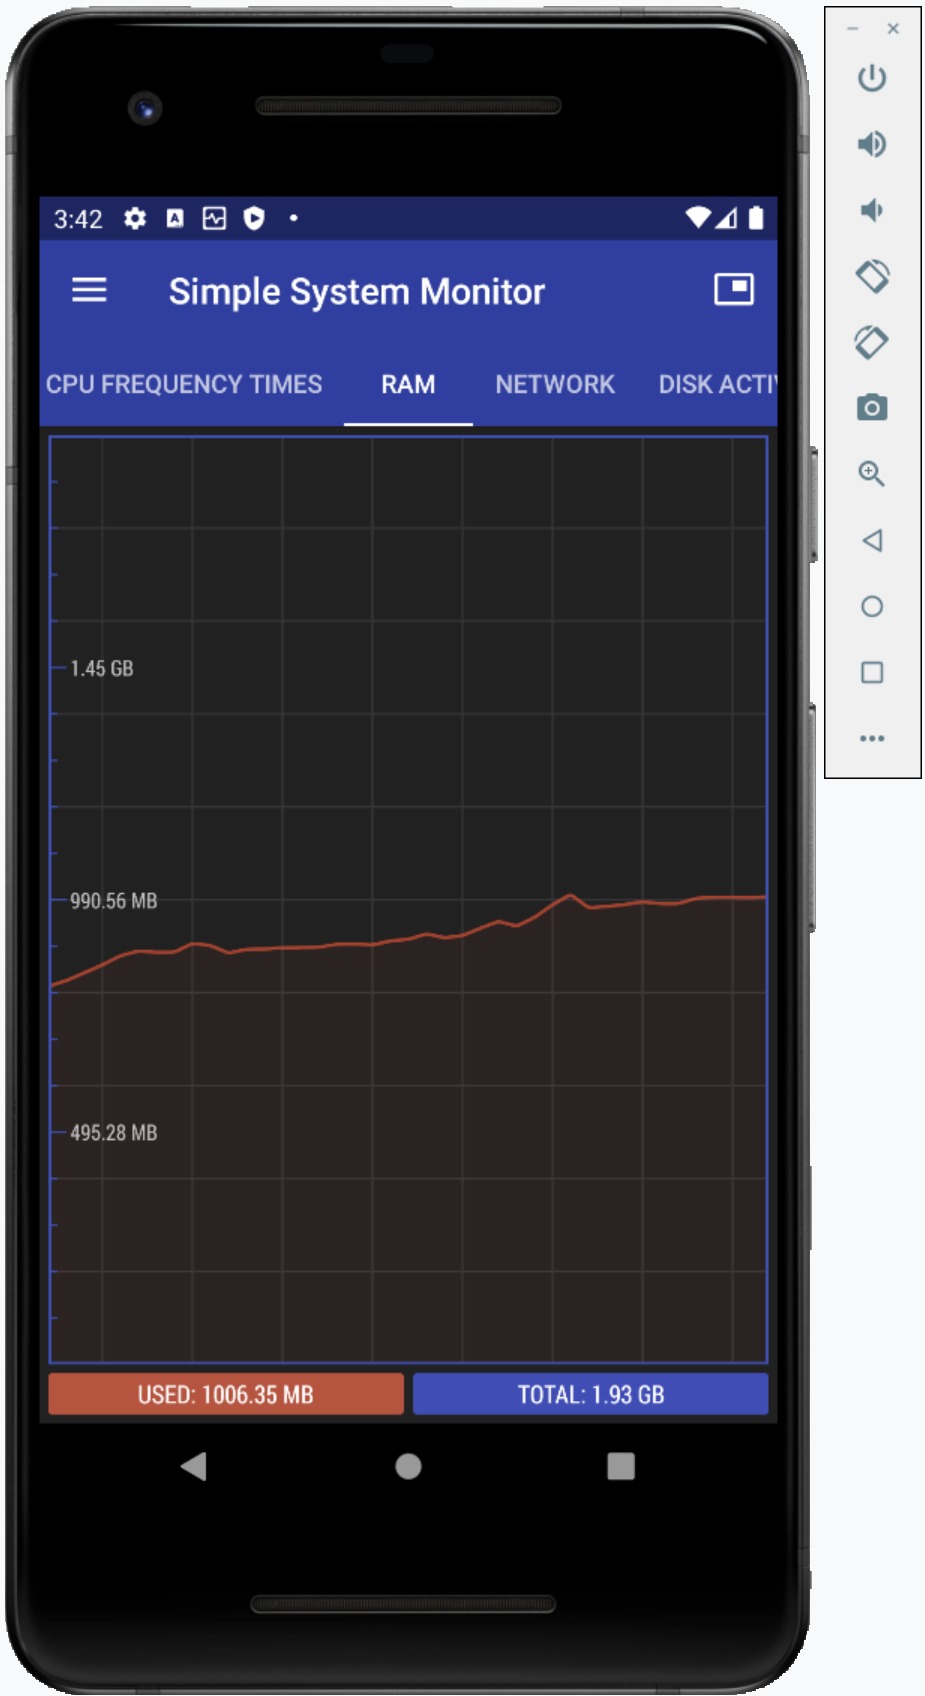
\includegraphics[width=4cm]{michael17.png}
\begin{minipage}{\linewidth}
\begin{wrapfigure}{r}{0.4\textwidth}
\centering
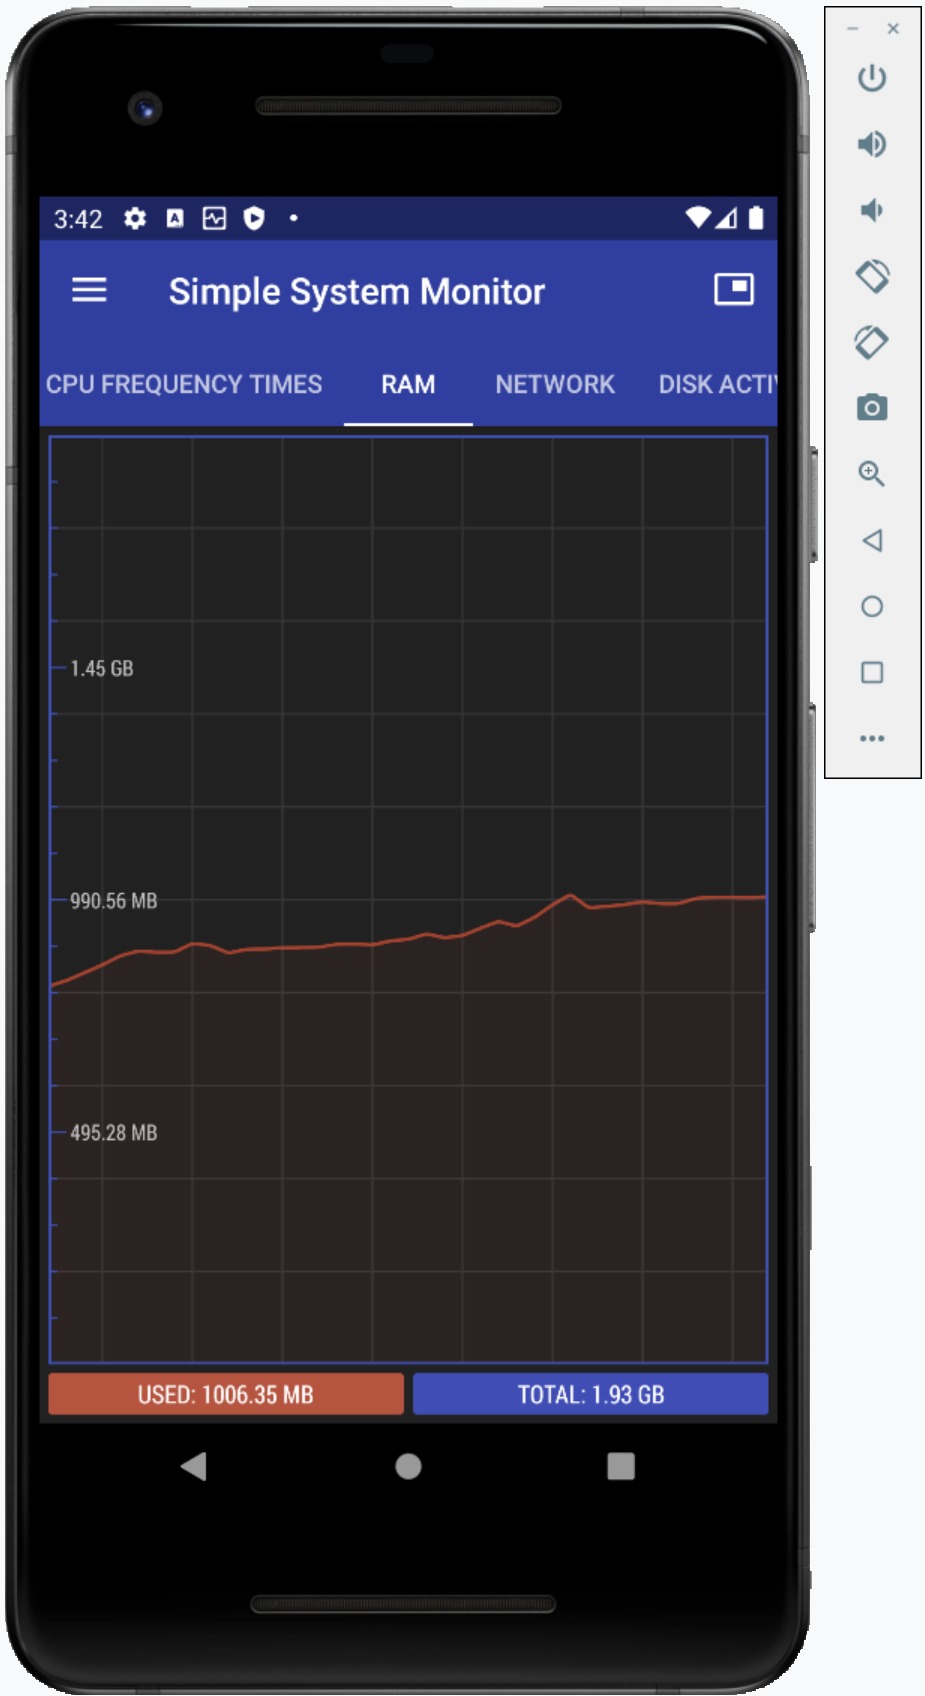
\includegraphics[scale=0.15]{michael17.png}
\end{wrapfigure}
~\\
~\\
~\\
~\\
~\\
~\\
~\\

Running the legitimate application until user interaction was possible, which is to say after boot-up and loading time, another screenshot has been made of the used RAM. The used memory shot up to more or less 1006MB of data. This means that the application used about 215MB of data. This is ordinary for an application such as this. Shutting down the application the used RAM went back down to about 820MB. This most likely consists of cached data.
\end{minipage}
~\\
~\\
~\\
~\\
~\\
~\\
~\\
~\\
~\\
~\\
~\\
~\\
~\\

%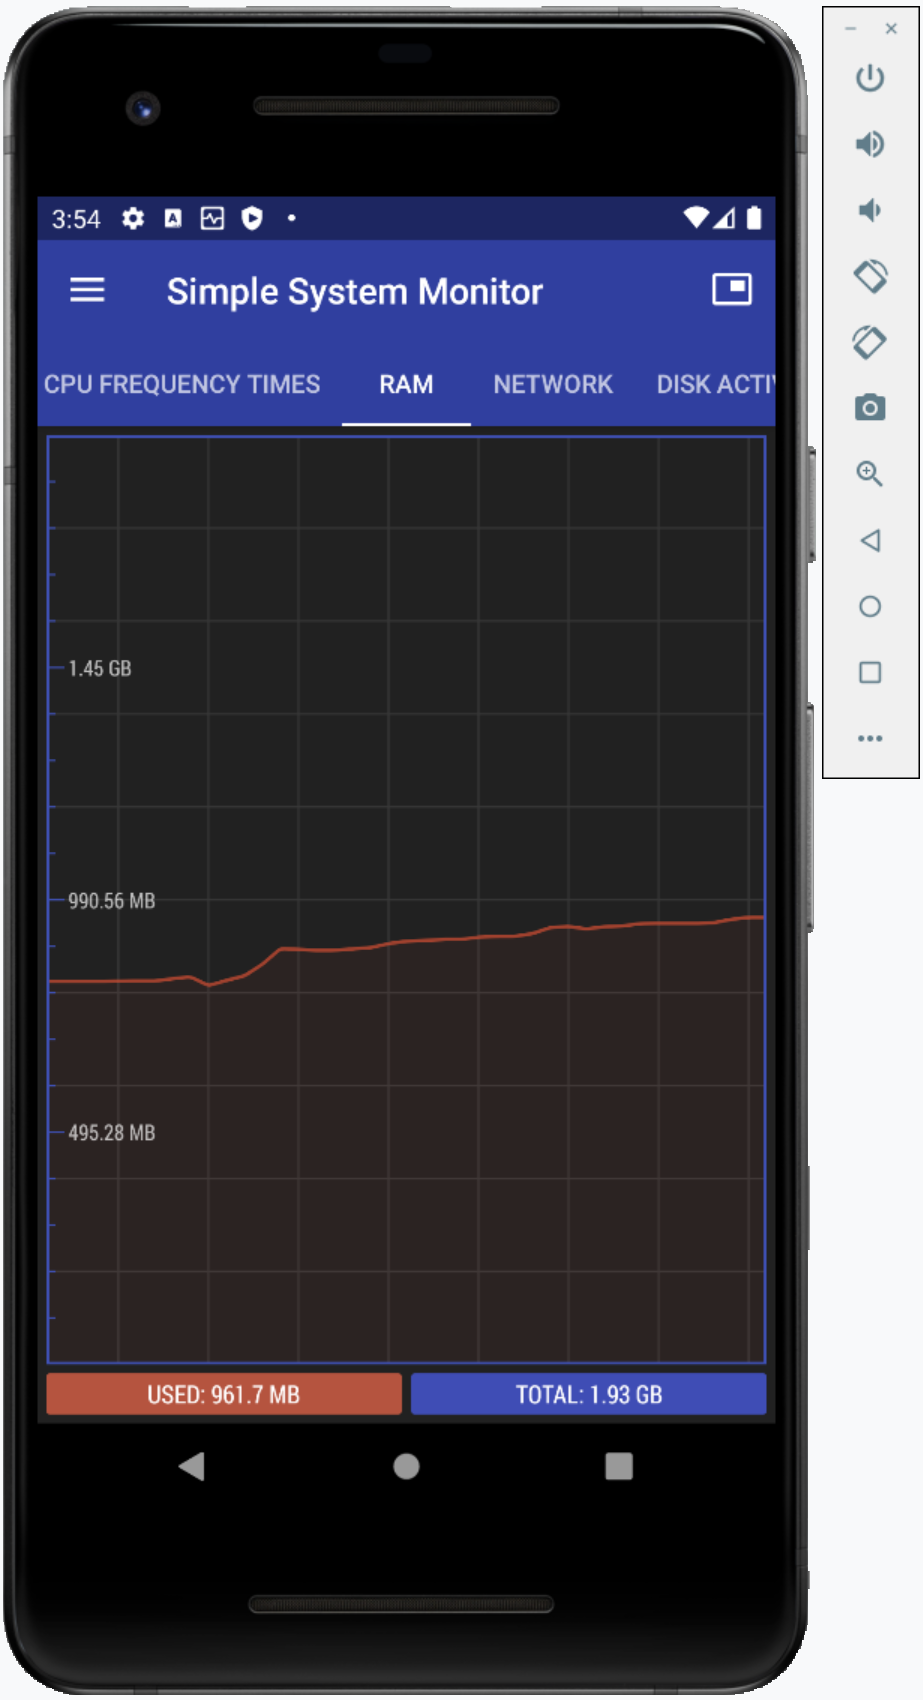
\includegraphics[width=4cm]{michael18.png}
\begin{minipage}{\linewidth}
\begin{wrapfigure}{l}{0.4\textwidth}
\centering
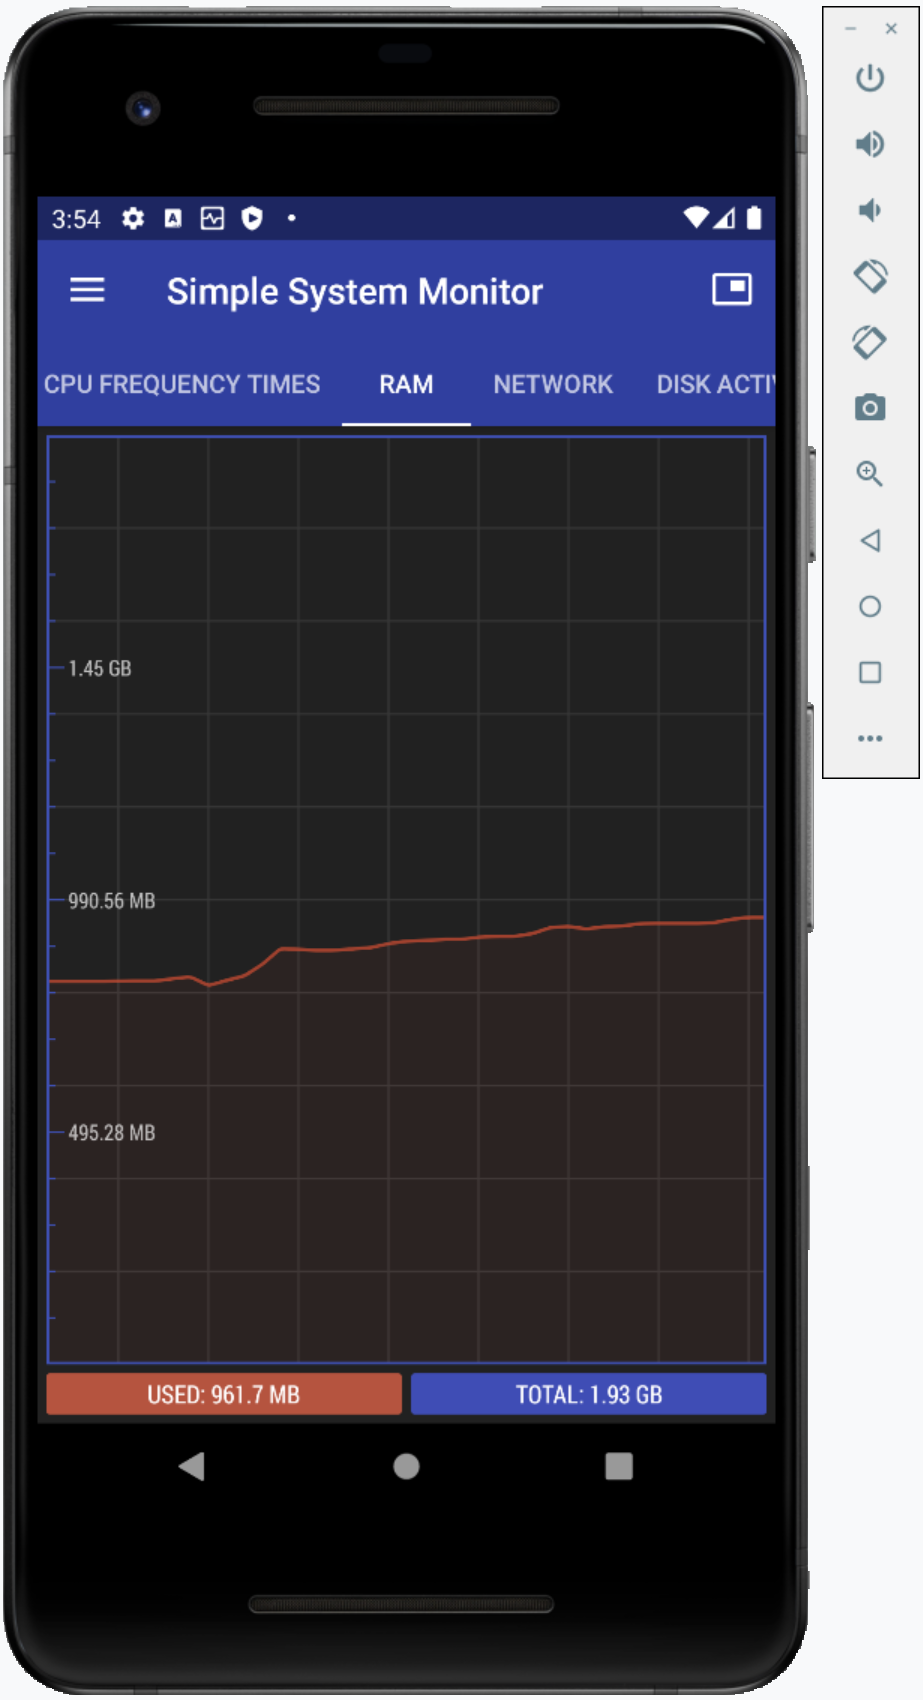
\includegraphics[scale=0.15]{michael18.png}
\end{wrapfigure}
~\\
~\\
~\\
~\\
~\\
~\\
~\\

This was the RAM benchmark of the malicious application. As can be seen, the data went up to about 960MB. Even after several tests, the malicious application used less RAM than the legitimate one. Why this one is more optimized than the real one is as of yet unknown, but perhaps it is possible to find the answer within the code after thorough searching. This version of the application used about 170MB of data. Which means a decrease to about 79% of the original.
\end{minipage}

\newpage
\subsection{Countermeasures and detection}

\subsubsection{Preventive measures}

The simplest way to avoid installing malicious apps would be to not download any APK files from the internet, instead using the Google Play Store, or alternatively for iPhone users the App Store. Even then, caution is advised. It is important to note what kind of permissions an application requires to install and run. A malicious application would most likely require more or unusual permissions. Another way of verifying the legitimacy of an application is to compare its hash or size, though size is not always a reliable measure, with one of a trusted source. Knowing what sources to trust is key to security in general. Keeping your phone or your phone’s software up to date is recommended as well. Lastly, since Android is open-source, the user is free to do whatever they desire with it. This causes complications for users who are not as well-versed in technology or phone software. Keeping users up to date with this kind of technology, and spreading awareness would reduce the amount of people who have been targeted by a huge amount.

\subsubsection{Detective measures}

There are two large indicators to identify the malicious application. The first being the mis-matched icons. Exceptional about this is that the app doesn’t need to be running to identify it. The second indicator is during start-up. If there is a message in Arabic which pops up, it is a fake application. Since this application is not all that dangerous, there is no harm in this. However, for other applications this method is not recommended: it could lead to an application running malicious code. Preventive measures still apply at this point, such as verifying the legitimacy of an app by hash or size, or by checking the source of the application.
\subsubsection{Reactive measures}

If the application is already installed it is recommended to remove it. Whatever the case, do not run the application. In the case of this app, uninstalling the software would work, but in other cases applications might be harder to remove or have installed additional malicious software. In that case it might be a good idea to restore a back-up. Both iOS and Android support and even recommend this feature, by use of iCloud or Google Drive. If the device becomes inaccessible, it might be necessary to run the device in safe mode. This way it could still be booted and the application could be removed.
\subsubsection{YARA rule set}

A simple way to filter this application is to create a YARA rule that detects if the string “www.farsroid.com” is present, and to specifically filter this app it is also useful to declare that the application size is below 40MB. Since the malicious version is smaller than the official one, and the official version is likely going to add updates such as extra levels or limited time events, the real app is likely to only get bigger. However, this condition could easily be removed so that the only requirement is that the string “www.farsroid.com” is present, to filter all apps made by this malicious developer.
\begin{verbatim}

rule filterfarsroidapps1
{
    meta:
        description = “Filter farsroid apps under 40MB”
        author = “Michael Francis”
        date = “2021/11/24”
    strings:
        $text_string_1 = "www.farsroid.com"
    condition:
        $text_string_1 and filesize < 40MB
}

\end{verbatim}

Or alternatively the filter without the size requirement:
\begin{verbatim}

rule filterfarsroidapps2
{
    meta:
        description = “Filter farsroid apps”
        author = “Michael Francis”
        date = “2021/11/24”
    strings:
        $text_string_1 = "www.farsroid.com"
    condition:
        $text_string_1
}

\end{verbatim}



\newpage
\section{'DHL Express Mobile' Application Analysis by Rafael}

The application that was analyzed in this chapter had the name 'DHL'.
The application was found on \href{https://koodous.com/apks/38ff459a46e9ea6d63a83c1eddb640626fef562cd1bcb0ab3823c4770d07d0fb}{Koodous} with the version \texttt{1.0} and package name \texttt{com.ru.dhl}, the size was \texttt{2.7 MB}.
The same package name did not exist on the Google Play Store. However, an application with the same icon was found \href{https://play.google.com/store/apps/details?id=com.dhl.exp.dhlmobile}{here}. It has the version \texttt{2.7.0}, package name \texttt{com.dhl.exp.dhlmobile} and a size of \texttt{25 MB}.

The application found on Koodous and the application found on the Google Play Store will hereinafter be referred to as 'Malicious application' and 'Original application' respectively.

\newpage
\subsection{VirusTotal summary}

VirusTotal indicated that the malicious application was marked by 33/63 security vendors as malicious, 
and that the original application was marked by 0/60 security vendors as malicious.

The malicious application was primarily marked as a Banker. 
A banker is generally an application that attempts to steal banking information in order to steal the users money.
If it was not marked as a banker it was either marked as a Trojan or a non repeating name.
This was the full list


\begin{tabular}{ |l|l| }
    \hline
    \textbf{Vendor} & \textbf{Detection} \\
    
    \hline
        Ad-Aware    &   Trojan.GenericKD.37488882 \\
    \hline
        Alibaba     &   TrojanSpy:Android/Banker.66c12705 \\
    \hline
        Antiy-AVL   &   Trojan/Generic.ASMalwAD.5B \\
    \hline
        Arcabit     &   Trojan.Generic.D23C08F2 \\
    \hline
        Avast-Mobile    &   APK:RepSandbox [Trj] \\
    \hline
        Avira (no cloud)    &   ANDROID/Spy.Banker.YD.Gen \\
    \hline
        BitDefender     &   Trojan.GenericKD.37488882 \\
    \hline
        BitDefenderFalx     &   Android.Trojan.Banker.WS \\
    \hline
        CAT-QuickHeal   &   Android.AbereBot.Af9d \\
    \hline
        Cynet   &   Malicious (score: 99) \\
    \hline
        DrWeb   &   Android.BankBot.852.origin \\
    \hline
        Emsisoft    &   Trojan.GenericKD.37488882 (B) \\
    \hline
        eScan   &   Trojan.GenericKD.37488882 \\
    \hline
        ESET-NOD32  &   A Variant Of Android/Spy.Banker.AZU \\
    \hline
        F-Secure    &   Malware.ANDROID/Spy.Banker.YD.Gen \\
    \hline
        FireEye     &   Trojan.GenericKD.37488882 \\
    \hline
        Fortinet    &   Android/AbereBot.A!tr \\
    \hline
        GData   &   Trojan.GenericKD.37488882 \\
    \hline
        Gridinsoft  &   Trojan.U.Banker.oa \\
    \hline
        Ikarus  &   Trojan.AndroidOS.Banker \\
    \hline
        K7GW    &   Spyware ( 005817811 ) \\
    \hline
        Kaspersky   &   HEUR:Trojan-Banker.AndroidOS.AbereBot.a \\
    \hline
        Kingsoft    &   Android.Troj.tn-banker.azu.(kcloud) \\
    \hline
        Lionic  &   Trojan.AndroidOS.AbereBot.C!c \\
    \hline
        MAX     &   Malware (ai Score=100) \\
    \hline
        McAfee  &   Artemis!4778ACA48D17 \\
    \hline
        McAfee-GW-Edition   &   Artemis!Trojan \\
    \hline
        Microsoft   &   TrojanSpy:AndroidOS/Banker.GV!MTB \\
    \hline
        Symantec    &   Trojan.Gen.MBT \\
    \hline
        Symantec Mobile Insight     &   AppRisk:Generisk \\
    \hline
        Tencent     &   A.privacy.AnubisTrojanBanking \\
    \hline
        Trustlook   &   Android.Malware.Trojan \\
    \hline
        ZoneAlarm by Check Point    &   HEUR:Trojan-Banker.AndroidOS.AbereBot.a \\
    \hline
\end{tabular}

\newpage
\subsubsection{Permission requests}
\subsubsubsection{Malicious application}
The malicious application requested the following permissions:

\texttt{android.permission.ACCESS\_NETWORK\_STATE}
\newline \texttt{android.permission.ACCESS\_WIFI\_STATE}
\newline \texttt{android.permission.CALL\_PHONE}
\newline \texttt{android.permission.CHANGE\_WIFI\_STATE}
\newline \texttt{android.permission.FOREGROUND\_SERVICE}
\newline \texttt{android.permission.INTERNET}
\newline \texttt{android.permission.MODIFY\_AUDIO\_SETTINGS}
\newline \texttt{android.permission.READ\_CALL\_LOG}
\newline \texttt{android.permission.READ\_CONTACTS}
\newline \texttt{android.permission.READ\_PHONE\_STATE}
\newline \texttt{android.permission.READ\_PRIVILEGED\_PHONE\_STATE}
\newline \texttt{android.permission.READ\_SMS}
\newline \texttt{android.permission.RECEIVE\_BOOT\_COMPLETED}
\newline \texttt{android.permission.RECEIVE\_SMS}
\newline \texttt{android.permission.REQUEST\_DELETE\_PACKAGES}
\newline \texttt{android.permission.REQUEST\_IGNORE\_BATTERY\_OPTIMIZATIONS}
\newline \texttt{android.permission.SEND\_SMS}
\newline \texttt{android.permission.SHUTDOWN}
\newline \texttt{android.permission.UPDATE\_DEVICE\_STATS}
\newline \texttt{android.permission.WAKE\_LOCK}
\newline \texttt{android.permission.WRITE\_CALL\_LOG}
\newline \texttt{android.permission.WRITE\_CONTACTS}

\newpage
\subsubsubsection{Original application}
The original application requested the following permissions:

\texttt{android.permission.CALL\_PHONE}
\newline \texttt{android.permission.FLASHLIGHT}
\newline \texttt{android.permission.READ\_APP\_BADGE}
\newline \texttt{android.permission.READ\_EXTERNAL\_STORAGE}
\newline \texttt{android.permission.READ\_PHONE\_STATE}
\newline \texttt{android.permission.USE\_FINGERPRINT}
\newline \texttt{android.permission.WRITE\_EXTERNAL\_STORAGE}
\newline \texttt{com.anddoes.launcher.permission.UPDATE\_COUNT}
\newline \texttt{com.dhl.exp.dhlmobile.permission.C2D\_MESSAGE}
\newline \texttt{com.google.android.c2dm.permission.RECEIVE}
\newline \texttt{com.htc.launcher.permission.READ\_SETTINGS}
\newline \texttt{com.htc.launcher.permission.UPDATE\_SHORTCUT}
\newline \texttt{com.huawei.android.launcher.permission.CHANGE\_BADGE}
\newline \texttt{com.huawei.android.launcher.permission.READ\_SETTINGS}
\newline \texttt{com.huawei.android.launcher.permission.WRITE\_SETTINGS}
\newline \texttt{com.majeur.launcher.permission.UPDATE\_BADGE}
\newline \texttt{com.oppo.launcher.permission.READ\_SETTINGS}
\newline \texttt{com.oppo.launcher.permission.WRITE\_SETTINGS}
\newline \texttt{com.sec.android.provider.badge.permission.READ}
\newline \texttt{com.sec.android.provider.badge.permission.WRITE}
\newline \texttt{com.sonyericsson.home.permission.BROADCAST\_BADGE}
\newline \texttt{com.sonymobile.home.permission.PROVIDER\_INSERT\_BADGE}
\newline \texttt{me.everything.badger.permission.BADGE\_COUNT\_READ}
\newline \texttt{me.everything.badger.permission.BADGE\_COUNT\_WRITE}



\newpage
\subsection{Behavior analysis}

<what does the app behave like when installed and ran>

\newpage
\subsection{Network analysis}

<what does the network traffic look like>

\subsubsection{HTTP proxy analysis}

<what did the proxy reveal about the network traffic>

\subsubsection{Wireshark analysis}

<what did WireShark reveal about the network traffic>

\subsubsection{Reconnaissance [optional]}

<what was found using shodan.io>

\newpage
\subsection{Code analysis}

<interesting stuff found in code>

\newpage
\subsection{Process analysis}

<interesting stuff found in the process and memory, etc.>

\newpage
\subsection{Countermeasures and detection}

\subsubsection{Preventive measures}


<Measures to prevent installing this application>

\subsubsection{Detective measures}

<Measures to detect if this application is installed>

\subsubsection{Reactive measures}

<What to do if it is installed>

\subsubsection{YARA rule set}

<A YARA rule set created based on your findings>


\newpage
\section{<application name> Application Analysis by Tim}

<should include application name, version numbers, apk size>

\newpage
\subsection{VirusTotal summary}

<should include, how many times marked malicious, package name and any other interesting things>

\subsubsection{Permission requests}

<permissions requested by the app (can be found on virus total)>

\newpage
\subsection{Behavior analysis}

<what does the app behave like when installed and ran>

\newpage
\subsection{Network analysis}

<what does the network traffic look like>

\subsubsection{HTTP proxy analysis}

<what did the proxy reveal about the network traffic>

\subsubsection{Wireshark analysis}

<what did WireShark reveal about the network traffic>

\subsubsection{Reconnaissance [optional]}

<what was found using shodan.io>

\newpage
\subsection{Code analysis}

<interesting stuff found in code>

\newpage
\subsection{Process analysis}

<interesting stuff found in the process and memory, etc.>

\newpage
\subsection{Countermeasures and detection}

\subsubsection{Preventive measures}


<Measures to prevent installing this application>

\subsubsection{Detective measures}

<Measures to detect if this application is installed>

\subsubsection{Reactive measures}

<What to do if it is installed>

\subsubsection{YARA rule set}

<A YARA rule set created based on your findings>


% \bibliography{references} % DIT ZIJN VOORBEELDEN
% \begin{thebibliography}{9}
% \end{thebibliography}

\end{document}


% book:
% author (release year). \textit{title}\\
% Editors. Publisher.
